% Track 2 — drug repurposing report. Compile: latexmk -lualatex track2.tex (see scripts/compila_informes.py)
\documentclass[10pt]{article}
\usepackage{mvareport}
\renewcommand{\reporttrack}{TRACK 2 · DRUG REPURPOSING}
\renewcommand{\reportshort}{Allele-aware repurposing for \textit{BUB1B} MVA}
\hypersetup{pdftitle={Track 2: allele-aware drug repurposing for BUB1B mosaic variegated aneuploidy},pdfauthor={Agustín Pérez Castro (aperezcastro)}}

\defref{suij}{Suijkerbuijk et al.}{2010}\defref{bohers}{Bohers et al.}{2008}\defref{baker13}{Baker et al.}{2013}
\defref{baker11}{Baker et al.}{2011}\defref{baker04}{Baker et al.}{2004}\defref{sieben}{Sieben et al.}{2020}
\defref{north}{North et al.}{2014}\defref{wu}{Wu et al.}{2023}\defref{mckay}{McKay-Corkum et al.}{2023}
\defref{ontrac}{Chen et al.}{2015}\defref{maric}{Maric et al.}{2023}\defref{farr}{Farr et al.}{2024}
\defref{justice}{Justice et al.}{2019}\defref{mackenzie}{Mackenzie et al.}{2017}\defref{bakhoum}{Bakhoum et al.}{2018}
\defref{santaguida}{Santaguida et al.}{2017}\defref{xu}{Xu et al.}{2015}\defref{sanchez}{Sanchez et al.}{2018}
\defref{malumbres}{Malumbres}{2024}\defref{mangk}{Mangkalaphiban et al.}{2024}\defref{mcelroy}{McElroy et al.}{2013}
\defref{trzaska}{Trzaska et al.}{2020}\defref{ochiai}{Ochiai et al.}{2019}\defref{nishitani}{Nishitani-Isa et al.}{2019}
\defref{nakano}{Nakano et al.}{2024}
\defref{gupta}{Gupta et al.}{2024}\defref{hymes}{Hymes \& Warshaw}{2011}\defref{rangel}{Rangel et al.}{2009}
\defref{gordon}{Gordon et al.}{2018}
\defref{fajgenbaum}{Fajgenbaum et al.}{2019}\defref{tang}{Tang et al.}{2011}\defref{gale}{Gale et al.}{2004}
\defref{knip}{Knip et al.}{2000}\defref{bitterman}{Bitterman et al.}{2002}\defref{donnelly}{Donnelly et al.}{2014}\defref{bonatti}{Bonatti et al.}{1998}
\defref{milan}{González-Blanco et al.}{2026}\defref{dertinger}{Dertinger et al.}{2003}\defref{baig}{Baig et al.}{2020}
\defref{mengel}{Mengel et al.}{2021}\defref{sayin}{Sayin et al.}{2014}\defref{wiel}{Wiel et al.}{2019}
\defref{dertinger11}{Dertinger et al.}{2011}

\begin{document}

\reportheader{Rare Disease, Real Kid · MVA Hackathon 2026 · Track 2 report}
{Allele-aware drug repurposing for \textit{BUB1B} mosaic variegated aneuploidy}
{Three evidence streams, a patient-aware safety model, and a ranking that let the evidence change our minds}
{Agustín Pérez Castro (\texttt{aperezcastro}, individual)\enspace·\enspace October 2026\\
Code: \href{https://github.com/aperezcastro/hackaton-genetico}{github.com/aperezcastro/hackaton-genetico}, \code{scripts/t2/} (CC BY 4.0)}
{All proposals are hypotheses to be tested, not treatment advice. Every decision about this child's care belongs to
their clinical team. Only gene-, pathway- and drug-level public data were used.}

\begin{keybox}[title={Recommendations at a glance}]
\tablefont
\begin{tabularx}{\linewidth}{@{}P{2.55cm}P{5.1cm}L@{}}
\textbf{Tier 0 · act now} & \textbf{Safety note} for the clinical team: drugs to discuss and monitor (never to drop a curative regimen), growth hormone, NAD\textsuperscript{+} supplements, HSP90 inhibitors; paediatric label items for every candidate & MVA case reports + mouse heart data + connectivity + FDA labels; its own risk is under-treatment, which is why it advises discussion, not substitution\\
\textbf{Tier 0 · measure} & \textbf{BUBR1 immunoblot} in the child's cells, and \textbf{\%MN-RET} in blood & the blot decides the allele class and so whether a corrective drug can exist; \%MN-RET is the first measure of this disease's activity in blood (never made in MVA), then a recent error rate on a weeks timescale\\
\textbf{Tier 1 · experiment} & \textbf{Intermittent dasatinib}, to be tested first in the published BubR1 allelic mouse & highest-scoring approved drug (narrowly ahead of ruxolitinib), and the only top candidate whose direction is tumour-suppressive; genetic senolysis delayed MVA-like phenotypes in BubR1 mice; no senolytic drug tested in that model\\
\textbf{Tier 2 · gated} & \textbf{An NAD\textsuperscript{+} precursor} (niacin; nicotinamide scores the same but inhibits sirtuins) to stabilise the hypomorphic protein & becomes the top-ranked option if the blot confirms the low-abundance class \emph{and} the child is in documented remission (rhabdomyosarcoma depends on NAMPT/NAD\textsuperscript{+})\\
\textbf{Tier 3 · conditioned} & \textbf{Low-dose sirolimus} for muscle loss, \textbf{with \%MN-RET as a safety readout} & mTORC1–sarcopenia link is from monoallelic mice; rapamycin was aneugenic in one in-vitro study; adding temsirolimus to chemotherapy raised myelotoxicity in paediatric RMS\\
\textbf{Tier 4 · biomarker-gated} & \textbf{JAK inhibitors}, only if an interferon signature is measured in the child & class-consistent reversal of the knockout signature, but not a top hit; may impair immune clearance of aneuploid cells\\
\textbf{Declined} & \textbf{Proteostasis amplifiers} (arimoclomol, sodium phenylbutyrate) and antioxidants & the lever is real, but raising HSF1 is a documented aneuploidy-\emph{tolerating} event: it makes chromosomally abnormal cells viable\\
\textbf{Closed (for now)} & Read-through of the nonsense allele & on current evidence: UGA-A context (a two-feature reading, not the published predictor) + NMD; ataluren discredited; the compounds that correct UGA are unapproved, and gentamicin reads through weakly and is nephrotoxic
\end{tabularx}
\end{keybox}

\noindent\statnum{2 facts}{(allele class, remission) would move a corrective drug from \#8 to \#1}\hfill
\statnum{0}{registered clinical trials for MVA (ClinicalTrials.gov)}\hfill
\statnum{32}{BUB1B-knockout signatures analysed (20 cell lines)}\hfill
\statnum{132}{MVA publications screened for treatments}

\section{Summary}

The child carries a \textbf{null} \gene{BUB1B} allele (p.Leu737*, UGA nonsense, NMD predicted) and a
kinase-domain missense allele (p.Asn1002Lys), as established in Track~1. The mechanism is \textbf{partial loss of
function}: the SAC is dosage-sensitive \citep{bohers}, and more BUBR1 protects against aneuploidy and cancer in
vivo \citep{baker13}, so modest gains in functional BUBR1 should help and drugs that add mitotic or genotoxic
stress should be avoided (Figure~\ref{fig:mecanismo}).

\textbf{What we do not know, and what it costs.} \citet{suij} separate MVA alleles into two classes: those that
lower BUBR1 abundance and those that impair its function at normal abundance. Which class p.Asn1002Lys belongs to
has never been measured. The prior favours low abundance --- every disease-associated substitution tested in
or near the kinase domain was 5--10$\times$ less abundant, and the known stable-but-dysfunctional alleles lie outside that domain --- so
we weight it 0.75, not 1. We carry both scenarios explicitly (§\ref{sec:alelo}) rather than assert the convenient
one: the corrective NAD\textsuperscript{+} line loses a quarter of its mechanistic fit, and one immunoblot becomes
the gate for it.

We combined three independent evidence streams in an open, reusable pipeline (Figure~\ref{fig:metodo}):
\begin{enumerate}
\item \textbf{Literature.} A curated, PMID-cited knowledge base of seven therapeutic lines plus a safety card, in which
  contrary evidence is scored and counts against us.
\item \textbf{Connectivity.} The consensus transcriptional signature of \gene{BUB1B} knockout (32 CRISPR signatures,
  20 cell lines, LINCS L1000), queried against the LINCS chemical-perturbation signatures (the 1,000 most
  significant hits per direction).
\item \textbf{Patient-aware safety.} FDA label text mined automatically and matched against the child's own phenotype
  (cancer predisposition, nephrocalcinosis, muscle atrophy, short stature), plus curated literature risks that no
  label records.
\end{enumerate}

\textbf{The mechanism-matched candidate exists, and we name it first:} an NAD\textsuperscript{+} precursor
(niacin), which is predicted to act on the defect itself by keeping the hypomorphic BUBR1 from being degraded (H1). We do not rank
it first today, for two reasons that are facts about this child and can be measured, not gaps in the
literature: whether the missense allele is of the low-abundance class (one immunoblot), and whether the child is in
remission (their tumour depends on NAD\textsuperscript{+}).

\textbf{The main result is a decision rule, not a single drug} (§\ref{sec:ejes}). We classify every line by what it
does to a chromosomally unstable cell --- \textbf{correct} fewer missegregation events, \textbf{clear} the abnormal
cells, \textbf{tolerate} help them cope. Under today's uncertainty the best-supported approved option,
\textbf{intermittent dasatinib}, is on the \emph{clear} axis: it ranks first, narrowly ahead of the JAK inhibitor ruxolitinib (0.73 vs 0.72; first in 42\,\% and 38\,\% of all
robustness draws), and it is the only top candidate whose direction is tumour-suppressive. The corrective
NAD\textsuperscript{+} line ranks eighth, held back by two named facts about this child: the unmeasured allele
class and the rhabdomyosarcoma's dependence on NAD\textsuperscript{+}. \textbf{If the clinical team establishes
either one, an NAD\textsuperscript{+} precursor rises to third; with both, it ranks first.} The two
\emph{tolerate} lines (mTOR and JAK inhibitors) share a different concern: both can blunt the immune clearance of
aneuploid cells, and in a cancer-predisposition syndrome a premalignant clone is an aneuploid cell too.

The second result is how much the evidence \textbf{changed our own plan} (Figure~\ref{fig:cambio}).
\begin{itemize}
\item Our initial lead, nicotinamide, fell from second to ninth (niacin, now the line's preferred precursor, is eighth): rhabdomyosarcoma, this child's tumour,
  depends on the NAD\textsuperscript{+} pathway it would feed, and nicotinamide itself inhibits sirtuins.
\item The read-through line was closed, on current evidence, by an allele-level analysis of the stop codon.
\item The best human senolytic trial missed its primary endpoint, so senolysis became an experiment to run rather
  than a treatment to propose.
\item Sirolimus, once our top-scoring drug, fell to tenth: the mTORC1--sarcopenia link it rested on comes from
  monoallelic mice, rapamycin was aneugenic in one in-vitro study \citep{bonatti}, and adding the mTOR inhibitor
  temsirolimus to chemotherapy raised myelotoxicity in paediatric RMS \citep{gupta}.
\item A commonly proposed alternative for this genotype --- proteostasis amplification ---
  was added as a line and then declined on the evidence, rather than left unmentioned (§\ref{sec:h7}).
\item A blind adversarial review of an earlier draft showed that our previous headline depended on two hand-set
  inputs and on harms counted twice (once against the evidence, once against safety). We separated the two in the
  model, widened the robustness analysis, and replaced that headline with the decision rule above.
\end{itemize}

\textbf{Impact beyond this child.} The safety card, the screen of every published MVA case and the knockout
signature are not specific to these two alleles; they apply to anyone with MVA1. We also propose a blood
measurement --- micronucleated reticulocytes (\%MN-RET) --- that has \textbf{never been made in anyone with MVA}. Its
first use is not about drugs: it would be the first quantitative readout of this disease's activity in blood, from
a routine draw, against a published paediatric reference range. That is a diagnostic and natural-history
observation for every MVA patient, and it can falsify the disease model before anyone is treated. Only then does it
become an endpoint that reports a \textbf{recent error rate on a weeks timescale}, with a one-page protocol and the
power calculation that says what it can and cannot resolve (§\ref{sec:medir}). \textbf{Innovation:} the therapeutic-axis model and the decision rule it yields; a
\textit{negative} output (what not to give); safety that goes beyond drug labels; an evidence model that scores
target validation below demonstrated benefit; and an allele-class uncertainty carried explicitly into the score
instead of being resolved by assumption.

\begin{figure}[htbp]
\centering
\begin{tikzpicture}[scale=0.94, transform shape, font=\sffamily\scriptsize, node distance=3mm and 6mm,
  st/.style={draw=rule, fill=white, rounded corners=2pt, align=center, inner sep=3pt, text width=#1, minimum height=7mm},
  st/.default=2.4cm, fl/.style={-{Stealth[length=1.8mm]}, draw=ink2, line width=0.6pt},
  lev/.style={fill=#1!14, text=#1!75!black, rounded corners=2pt, font=\sffamily\scriptsize\bfseries, inner sep=2.2pt, align=center},
  lk/.style={draw=#1!60, line width=0.6pt, dashed}]
  \node[st=2.85cm, draw=accent] (a1) {\textbf{Allele 1} · p.Leu737*\\UGA stop · NMD\\\textcolor{ink2}{no protein}};
  \node[st=2.85cm, draw=brand, below=7mm of a1] (a2) {\textbf{Allele 2} · p.Asn1002Lys\\kinase-domain missense\\\textcolor{critical}{\textbf{class not measured:}}\\\textcolor{ink2}{A unstable \textbar{} B dysfunctional}};
  \node[st=2.2cm, fill=panel, right=9mm of a1, yshift=-7mm] (low) {\textbf{Low BUBR1}\\below the $\sim$50\,\%\\dosage threshold};
  \node[st=2.3cm, right=7mm of low] (mis) {\textbf{Weak checkpoint}\\chromosome\\missegregation};
  \node[st=2.6cm, right=9mm of mis, yshift=17mm] (c1) {micronuclei \arr\ cGAS–STING\\\textbf{interferon / NF-$\kappa$B}};
  \node[st=2.6cm, below=2.2mm of c1] (c2) {\textbf{senescence} + SASP\\progeroid features};
  \node[st=2.6cm, below=2.2mm of c2] (c3) {\textbf{mTORC1} hyperactivity\\sarcopenia};
  \node[st=2.6cm, below=2.2mm of c3] (c4) {\textbf{aneuploid cells}\\tumours (RMS, Wilms)};
  \draw[fl] (a1.east) -- ++(4mm,0) |- (low.west);
  \draw[fl] (a2.east) -- ++(4mm,0) |- (low.west);
  \draw[fl] (low) -- (mis);
  \foreach \c in {c1,c2,c3,c4} \draw[fl] (mis.east) -- ++(4mm,0) |- (\c.west);
  \node[lev=critical, above=2mm of a1] (h2) {H2 read-through · \textit{closed}};
  \node[lev=brand, below=2mm of a2] (h1) {H1 stabilise (NAD\textsuperscript{+}/SIRT2) · H7 proteostasis\\\textit{both exist only under scenario A}};
  \node[lev=violet, right=2mm of c1] (h6) {H6 JAK};
  \node[lev=aqua, right=2mm of c2] (h4) {H4 senolysis};
  \node[lev=accent, right=2mm of c3] (h3) {H3 mTORC1};
  \node[lev=muted, right=2mm of c4] (h5) {H5 \textit{not pursued}};
  \node[lev=critical, below=3mm of mis] (s1) {S1 avoid extra\\mitotic or genotoxic stress};
  \draw[lk=critical] (s1) -- (mis);
\end{tikzpicture}
\caption{Disease mechanism and where each therapeutic line acts. Each allele has its own lever (H1 and H7 on the
missense allele, H2 on the nonsense one), and the two missense-allele levers are conditional on an allele class nobody has measured
(§\ref{sec:alelo}); the other lines act on druggable consequences of chronic missegregation; the safety card (S1)
acts on the weak checkpoint itself. Colour identifies the line, not the axis; for the axes see §\ref{sec:ejes}.}
\label{fig:mecanismo}
\end{figure}

\section{Disease mechanism model}
Table~\ref{tab:mecanismo} summarises the mechanism, level by level, with its evidence.
\begin{table}[tbp]\tablefont
\begin{tabularx}{\linewidth}{@{}P{2.3cm}LP{3.4cm}@{}}
\toprule\thead{Level} & \thead{Fact} & \thead{Evidence}\\\midrule
Gene & \gene{BUB1B} encodes BUBR1, a core subunit of the mitotic checkpoint complex that inhibits APC/C–CDC20 until all kinetochores are attached; it also stabilises kinetochore–microtubule attachments & \citealp{baker13}, \pmid{23242215}\\
Allele 1 & nonsense p.Leu737*, exon 17/23, NMD; truncating MVA alleles yield no transcript & \citealp{suij}, \pmid{20516114}\\
Allele 2 & kinase-domain missense. \textbf{Class not measured} (§\ref{sec:alelo}): low-abundance (prior 0.75: every disease-associated substitution tested in or near the kinase domain was 5--10$\times$ less abundant) or stable-but-dysfunctional (0.25: known examples lie outside the kinase domain) & \citealp{suij}\\
Structure & Asn1002 is a high-confidence (AlphaFold pLDDT 91), largely buried residue packing against the kinase C-lobe, 12~Å from the MVA1 allele L1012P; a longer, charged Lys could destabilise the fold (consistent with scenario A, not proof of it) & \code{scripts/t2/estructura.py}\\
Dosage & aneuploidy appears below $\sim$50\,\% residual BUBR1; graded effects across 8–77\,\% & \citealp{bohers}, \pmid{18932004}\\
Rescue logic & ectopic BUBR1 restores the checkpoint in MVA patient cells; transgenic BubR1 overexpression reduces aneuploidy and cancer in mice & \citealp{suij,baker13}\\
Cellular response & knockout: interferon-$\alpha/\gamma$, NF-$\kappa$B and p53 programmes up, proliferation down (§\ref{sec:cmap}), consistent with micronuclei sensed by cGAS–STING & \citealp{mackenzie}, \pmid{28738408}; \citealp{santaguida}, \pmid{28633018}\\
Phenotype drivers & aneuploidy leads to tumours, senescence + SASP (sarcopenia, lipodystrophy, cataract) and growth failure & \citealp{baker04,baker11,sieben}\\
Genotype-specific & in a BubR1 allelic series, the truncating + kinase-domain missense genotype closest to this child (X753/L1002P; mouse L1002 = human L1012) \textbf{died prematurely}; the viable biallelic model (H/L1002P) shows the MVA spectrum; sarcopenia correlated with mTORC1 hyperactivity in mice carrying a \textbf{single} MVA allele & \citealp{sieben}, \pmid{31738183}\\
\textbf{Feedback loop} & \textbf{a prediction specific to this genotype.} Kinase-domain BUBR1 mutants need HSP90 to fold and are cleared by the proteasome without it; and aneuploid human cells are \emph{already} impaired in HSP90-dependent folding, with a compromised heat-shock response. If allele 2 is of the low-abundance class, aneuploidy erodes the chaperone reserve that the hypomorphic allele depends on, in the very cells that need it most: less BUBR1 $\rightarrow$ more aneuploidy $\rightarrow$ worse folding $\rightarrow$ less folded BUBR1 & \citealp{suij}, \pmid{20516114}; \citealp{donnelly}, \pmid{25205676}\\\bottomrule
\end{tabularx}
\caption{Disease mechanism model, level by level, with the evidence for each step.}\label{tab:mecanismo}\end{table}

\subsection{The one fact that would change everything, and we do not have it}
\label{sec:alelo}

\begin{cautionbox}[title={Two scenarios for p.Asn1002Lys, carried in parallel}]
\tablefont
\begin{tabularx}{\linewidth}{@{}P{2.3cm}LL@{}}
\toprule & \thead{A · low abundance} & \thead{B · stable, dysfunctional}\\\midrule
Precedents in the same study & I909T, L1012P, R727C, R814H, L844F: 5--10$\times$ less protein, turnover doubled, HSP90- and proteasome-dependent & Y155C (stable; restores alignment but not the checkpoint) and R550Q (stable) --- both \emph{outside} the kinase domain. The one stable kinase-domain substitution, Q921H, is a functionally normal passenger in \emph{cis} with the causal L844F\\
What the defect is & scarcity & the molecule itself\\
Consequence for therapy & abundance is the lever: forced re-expression of I909T and L1012P \emph{fully} restored the checkpoint, so there is nothing wrong with the protein except that there is too little of it. H1 is on-mechanism & stabilising it achieves nothing, and no approved drug restores the function. The actionable set collapses to the safety card and the downstream lines\\
Prior we assign & 0.75 & 0.25\\\bottomrule
\end{tabularx}
\end{cautionbox}

\noindent The kinase-domain position makes scenario A likely but not certain: this residue has never been
characterised, and the child's survival, where the mouse X753/L1002P died, might mean that p.Asn1002Lys keeps more function than L1012P. Three consequences follow.

\begin{enumerate}
\item \textbf{The uncertainty is priced into the mechanistic fit, not into the evidence.} The studies behind H1
  are exactly as strong as they were; what is uncertain is whether \emph{this} child is the kind of patient they
  apply to. So H1 gets $M = 0.8 \times 0.75 = 0.6$, while $E$ is left untouched. Putting it in the right term matters:
  it moves the NAD\textsuperscript{+} line down the ranking without pretending the underlying biology is weaker than it is.
\item \textbf{One experiment decides it}, and it is cheap: a BUBR1 immunoblot on the child's cells, with a
  cycloheximide chase if the level is low. That is rung~1 of the validation ladder (§\ref{sec:validacion}), and it
  is the gate for every restorative proposal here.
\item \textbf{The decision rule is pre-declared.} Residual full-length BUBR1 clearly below the parental carrier
  range, with accelerated turnover, supports scenario~A and opens H1 and H7. A level in the carrier range with
  normal turnover supports scenario~B and \textbf{closes} both, leaving tiers 0, 1, 3 and 4 --- none of which
  depends on the allele class.
\end{enumerate}

\section{Methods: the pipeline}
\label{sec:metodo}

\begin{figure}[htbp]
\centering
\begin{tikzpicture}[font=\sffamily\scriptsize, node distance=3mm and 8mm,
  st/.style={draw=#1, line width=0.7pt, fill=white, rounded corners=2pt, align=left, inner sep=4pt, text width=4.6cm},
  fl/.style={-{Stealth[length=1.8mm]}, draw=ink2, line width=0.6pt}]
  \node[st=brand] (lit) {\textbf{1 · Literature knowledge base}\\\code{hipotesis.yaml}: 7 lines + safety card; every
    item with a PMID, an evidence level and a role (support / contrary / harm)};
  \node[st=violet, below=of lit] (cm) {\textbf{2 · Connectivity} \code{cmap.py}\\32 BUB1B knockout signatures (LINCS
    L1000) \arr\ consensus \arr\ top 1,000 chemical signatures per direction; mimickers vs reversers};
  \node[st=aqua, below=of cm] (saf) {\textbf{3 · Patient-aware safety} \code{candidatos.py}\\ChEMBL + FDA labels + FDA
    NDC: approval, boxed warnings, paediatric forms \arr\ flags against the child's HPO risk profile};
  \node[draw=rule, fill=panel, rounded corners=2pt, align=left, inner sep=4pt, text width=4.3cm, right=12mm of cm] (sc)
    {\textbf{Transparent score}\\$0.30\,E + 0.25\,M + 0.20\,P + 0.25\,S$\\[1pt]
    E evidence · M mechanistic fit\\P paediatric feasibility · S safety\\[1pt]
    approved medicines only\\2,000 draws: weights, M $\pm$0.30, S $\pm$0.15};
  \node[draw=brand, fill=brand!10, rounded corners=2pt, align=left, inner sep=4pt, text width=4.3cm, below=4mm of sc] (ti)
    {\textbf{Clinical tiering by benefit–risk}\\tier 0 safety card \arr\ tiers 1–4 \arr\ closed lines};
  \draw[fl] (lit.east) -- ++(5mm,0) |- (sc.west);
  \draw[fl] (cm.east) -- (sc.west);
  \draw[fl] (saf.east) -- ++(5mm,0) |- (sc.west);
  \draw[fl] (sc) -- (ti);
\end{tikzpicture}
\caption{Three independent evidence streams feed one transparent score; the clinical tiering is then argued
explicitly. The connectivity stream is also used to challenge our own candidates, not only to find new ones.}
\label{fig:metodo}
\end{figure}

\textbf{Score components.}
\begin{itemize}
\item \textbf{E, evidence that the line works} (0–1): weight of the strongest supporting study, +0.1 per additional
  one (max +0.2), minus $0.3\times$ the weight of each contrary study (max $-0.3$), so that E does not depend on how
  hard we searched for contrary evidence. Evidence of \textbf{benefit} weighs human same gene 1.0, mouse same gene
  0.8, human other 0.7, cell same gene 0.5, mouse other 0.5, non-mammalian animal 0.4, cell other 0.3.
  \textbf{Target validation} (the pathway is disturbed, no benefit of modulating it shown) weighs 0.5 or 0.3, and
  \textbf{feasibility} in another disease (tolerated, no benefit for this mechanism) weighs 0.3. A pathway being
  active is not evidence that blocking it helps.
\item \textbf{M, mechanistic fit} to \textit{this} genotype (0–1, curated and justified in the YAML).
\item \textbf{P, paediatric feasibility}: label with paediatric use or dosing 1.0; label without 0.6; approved without a
  US label 0.5; supplement 0.35.
\item \textbf{S, patient-specific safety}: 1 $-$ 0.25 per boxed-warning flag $-$ 0.1 per warning flag, minus a
  \textbf{curated literature risk} for hazards no label records (max penalty 0.7). Evidence that a line could
  \emph{harm this child} lowers S only; it no longer also lowers E. The curated risks: the NAMPT dependency of
  rhabdomyosarcoma (H1, 0.35), aneuploidy tolerance (H7, 0.3), aneugenicity and paediatric myelotoxicity (H3, 0.2),
  weakened immune clearance of aneuploid cells (H6, 0.2).
\end{itemize}
Safety weighs as much as mechanism because this is a child with cancer predisposition. Connectivity is shown next to
the score but not inside it, because the signatures come from tumour cell lines after acute knockout.

\section{Results}

\subsection{Ranked candidates}
Only \textbf{approved medicines} are ranked, matching the Track~2 scope confirmed by the organisers (discussion \#5).
Quercetin, fisetin and nicotinamide riboside are dietary supplements and are listed but not ranked; ataluren was
removed on efficacy grounds (§\ref{sec:rt}).



\begin{table}[H]\sffamily\scriptsize
\begin{tabularx}{\linewidth}{@{}P{0.45cm}P{2.1cm}P{0.6cm}P{1.0cm}P{0.55cm}P{0.6cm}P{0.55cm}P{0.55cm}P{0.7cm}P{1.75cm}L@{}}
\toprule\thead{\#} & \thead{Drug} & \thead{Line} & \thead{Axis} & \thead{E} & \thead{M} & \thead{P} & \thead{S} & \thead{Score} & \thead{Paediatric form} & \thead{Key patient-specific flag}\\\midrule
1 & dasatinib & H4 & clear & 0.6 & 0.60 & 1.0 & 0.80 & \textbf{0.73} & oral suspension & pleural effusion, PAH, paediatric bone growth (label)\\
2 & ruxolitinib & H6 & tolerate & 0.9 & 0.40 & 1.0 & 0.60 & 0.72 & solid only & malignancy (oral label, no boxed warning); may weaken immune clearance\\
3 & tofacitinib & H6 & tolerate & 0.9 & 0.40 & 1.0 & 0.45 & 0.68 & oral solution & malignancy (boxed); may weaken immune clearance\\
4 & fedratinib & H6 & tolerate & 0.9 & 0.40 & 0.6 & 0.70 & 0.67 & solid only & malignancy; boxed encephalopathy (Wernicke; not a patient-risk flag, so not scored)\\
5 & arimoclomol & H7 & correct & 0.7 & 0.30 & 1.0 & 0.70 & 0.66 & solid only & \textbf{declined}: aneuploidy tolerance (§\ref{sec:h7})\\
6 & acetylcysteine & H7 & correct & 0.7 & 0.30 & 1.0 & 0.70 & 0.66 & oral/IV solution & \textbf{declined}: aneuploidy tolerance\\
7 & sodium phenylbutyrate & H7 & correct & 0.7 & 0.30 & 1.0 & 0.70 & 0.66 & pellets & \textbf{declined}: aneuploidy tolerance\\
8 & \textbf{niacin} & H1 & correct & 0.85 & 0.60 & 0.6 & 0.45 & 0.64 & oral solution & \textbf{NAMPT dependency of RMS}; label: myopathy, renal\\
9 & nicotinamide & H1 & correct & 0.85 & 0.40 & 0.6 & 0.65 & 0.64 & solid only & NAMPT dependency of RMS; inhibits sirtuins\\
10 & sirolimus & H3 & tolerate & 0.55 & 0.60 & 1.0 & 0.45 & 0.63 & oral solution & aneugenic in vitro; malignancy (boxed)\\
11 & baricitinib & H6 & tolerate & 0.9 & 0.40 & 0.6 & 0.45 & 0.60 & solid only & malignancy (boxed)\\
12 & everolimus & H3 & tolerate & 0.55 & 0.60 & 1.0 & 0.30 & 0.59 & dispersible tablet & malignancy, nephrotoxicity (boxed)\\
13 & hydroxychloroquine & H5 & clear & 0.3 & 0.40 & 1.0 & 0.70 & 0.57 & solid only & cell-line evidence only\\
14 & metformin & H5 & clear & 0.3 & 0.40 & 1.0 & 0.65 & 0.55 & oral solution & cell-line evidence only\\
15 & amlexanox & H2 & correct & 0.4 & 0.15 & 0.5 & 1.00 & 0.51 & solid only & UGA-A context + NMD (§\ref{sec:rt})\\\bottomrule
\end{tabularx}
\caption{Ranked approved medicines (full table with every column: \code{reports/t2/candidatos.md}). The
\emph{axis} column is the result that matters: see §\ref{sec:ejes}. Ties (5--7, 8--9) are listed in the knowledge
base's order. Nicotinamide is sold mostly as an over-the-counter vitamin; niacin is a prescription medicine.}
\end{table}

\begin{figure}[htbp]
\centering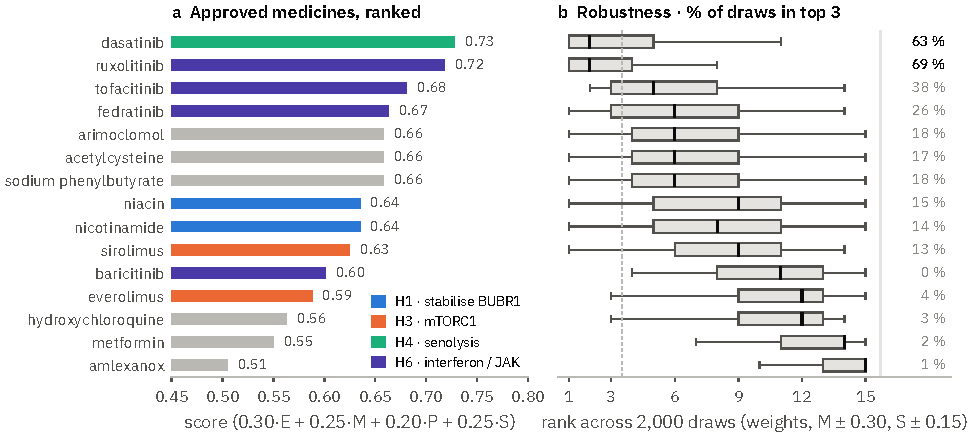
\includegraphics[width=\linewidth]{fig/t2_ranking.pdf}
\caption{\textbf{a}, Score of the 15 approved medicines, coloured by therapeutic line; grey marks the lines this
report does not propose (H2 closed, H5 not pursued, H7 declined). \textbf{b}, Rank distribution over 2,000 draws
that perturb the weights (Dirichlet), each line's mechanistic fit ($\pm$0.30) and each line's safety ($\pm$0.15),
with ties broken at random; right, share of draws in the top 3. Dasatinib (42\,\%) and ruxolitinib (38\,\%)
share most first places; the other JAK inhibitors and the H7 agents follow, which is why the clinical tiering, not the score, carries the
recommendation.}
\label{fig:ranking}
\end{figure}

The score is an input to, not a substitute for, the clinical reasoning. Dasatinib leads, and tier~1 frames it as
the one decisive, cheap experiment nobody has run rather than as a treatment. The JAK inhibitors score high on
evidence because JAK inhibition has shown clinical benefit in human type~I interferonopathies (a different
disease, so graded \emph{human\_other}), but low on fit; ruxolitinib leads them because its oral label carries
no boxed warning (unlike tofacitinib and baricitinib) and it has full paediatric feasibility (unlike fedratinib). They stay a biomarker-gated tier~4, because the interferon signature has never been measured in
any MVA patient. Sirolimus, first in an earlier draft, now ranks tenth (§\ref{sec:h3}). The dasatinib +
quercetin combination used in mouse studies includes a supplement, so we propose dasatinib as the approved agent
and test both arms preclinically.

\subsection{What each line does to an unstable cell, and what would change the answer}
\label{sec:ejes}

Ranking drugs by score answers ``which is best?''. It does not answer the question a clinician actually faces,
which is what the drug \emph{does} to a population of chromosomally unstable cells. We therefore label every line
with one of three axes, declared in the knowledge base alongside the mechanism rather than assigned after seeing
the ranking:

\begin{table}[H]\tablefont
\begin{tabularx}{\linewidth}{@{}P{1.6cm}LP{3.5cm}@{}}
\toprule\thead{Axis} & \thead{What it does} & \thead{Lines}\\\midrule
\textbf{correct} & fewer missegregation events: more functional BUBR1, so fewer errors are made & H1 (NAD\textsuperscript{+}/SIRT2), H2 (read-through), H7 (proteostasis)\\
\textbf{clear} & remove the cells that are already abnormal & H4 (senolysis), H5 (aneuploid-selective stress)\\
\textbf{tolerate} & leave the error rate alone and help the resulting cells cope & H3 (mTORC1), H6 (interferon/JAK)\\
\textbf{avoid} & do not add mitotic or genotoxic insult & S1 (safety card)\\\bottomrule
\end{tabularx}\end{table}

\begin{figure}[htbp]
\centering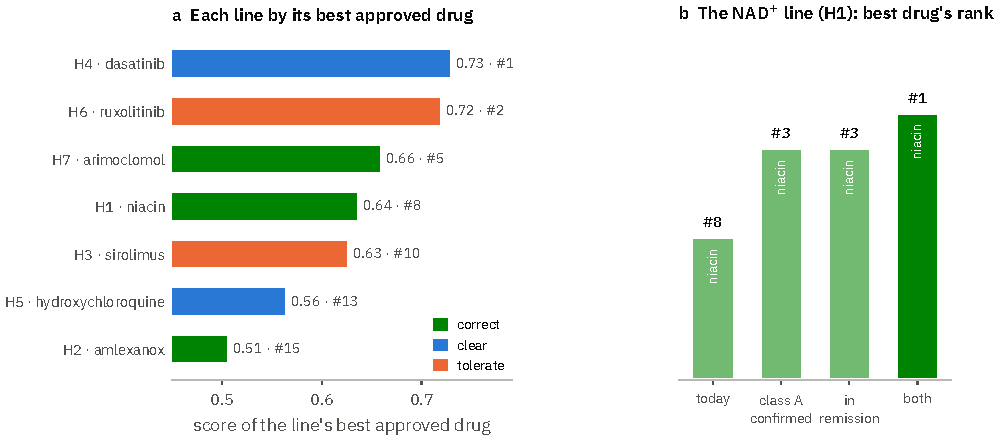
\includegraphics[width=\linewidth]{fig/t2_ejes.pdf}
\caption{\textbf{a}, Each therapeutic line placed by the score of its best approved drug, coloured by axis.
Summarised per line, not averaged over drugs: a mean over drugs would mostly report how many drugs we seeded per
line. \textbf{b}, The rank of the corrective NAD\textsuperscript{+} line's best drug under the two facts a clinical
team can establish.}
\label{fig:ejes}
\end{figure}

\textbf{No axis wins on the evidence; the corrective lines are each blocked by a different, nameable fact about
this child.} That is the useful statement, and it is checkable line by line:

\begin{table}[H]\tablefont
\begin{tabularx}{\linewidth}{@{}P{0.8cm}P{1.3cm}P{1.9cm}P{0.9cm}L@{}}
\toprule\thead{Line} & \thead{Axis} & \thead{Best drug} & \thead{Rank} & \thead{What blocks it}\\\midrule
H4 & clear & dasatinib & 1 & no senolytic ever tested in a BubR1 model; the best human senolytic RCT missed its primary endpoint\\
H6 & tolerate & ruxolitinib & 2 & may weaken the immune clearance of aneuploid cells; no interferon signature has been measured in any MVA patient\\
H7 & correct & arimoclomol & 5 & its mechanism \emph{is} aneuploidy tolerance (§\ref{sec:h7})\\
H1 & correct & niacin & 8 & allele class unmeasured; rhabdomyosarcoma depends on NAMPT/NAD\textsuperscript{+}\\
H3 & tolerate & sirolimus & 10 & aneugenic in vitro; temsirolimus added myelotoxicity in paediatric rhabdomyosarcoma\\
H5 & clear & hydroxychloroquine & 13 & cell-line evidence only; would also deplete normal mosaic tissue\\
H2 & correct & amlexanox & 15 & UGA-A stop context plus NMD; the compounds that correct UGA are unapproved\\\bottomrule
\end{tabularx}\end{table}

\textbf{Two measurements would move a corrective drug to the top.} Both concern H1 and both are things a clinical
team can establish; nothing else in the model changes.

\begin{table}[H]\tablefont
\begin{tabularx}{\linewidth}{@{}P{4.6cm}P{2.1cm}P{2.1cm}L@{}}
\toprule\thead{Scenario} & \thead{Best overall} & \thead{Second} & \thead{Best corrective drug (rank)}\\\midrule
As scored today & dasatinib & ruxolitinib & arimoclomol, declined (5)\\
Allele class A confirmed (rung-1 blot) & dasatinib & ruxolitinib & niacin (3)\\
Documented remission (NAMPT concern 0.35 $\rightarrow$ 0.10) & dasatinib & ruxolitinib & niacin (3)\\
\textbf{Both} & \textbf{niacin} & nicotinamide & \textbf{niacin (1)}\\\bottomrule
\end{tabularx}\end{table}

This is the opposite of a robustness claim, and we state it that way deliberately: the ranking \emph{is} sensitive
to these two inputs, which is exactly why the report's first recommendation is to measure them rather than to
prescribe. An earlier draft instead claimed that six of the seven best-scoring medicines sat on the
\emph{tolerate} axis and that this was ``not a weighting artefact''. A blind adversarial review showed it was: the
claim flipped when either of two curated H1 inputs was returned to its earlier value, and neither was inside the
robustness analysis. We now perturb mechanistic fit over $\pm$0.30 and safety over $\pm$0.15, break ties at random,
and publish the counterfactual table above instead of the claim.

\begin{cautionbox}[title={The hazard the axis makes visible}]
In a cancer-predisposition syndrome, \textbf{a premalignant aneuploid clone is an abnormal cell too}. A drug on the
\emph{tolerate} axis cannot distinguish a struggling but healthy aneuploid cell in muscle from a clone on its way to
a second malignancy; by construction, it helps both. That is explicit for H7, where the lever \emph{is} an
aneuploidy-tolerating mechanism \citep{donnelly}, and it is why H3 and H6 are proposed only against named morbidity
(muscle loss, inflammatory disease) with surveillance, never as chemoprevention. It is also why the safety note and
the measurement plan, not a prescription, are what we put first.
\end{cautionbox}

\begin{figure}[htbp]
\centering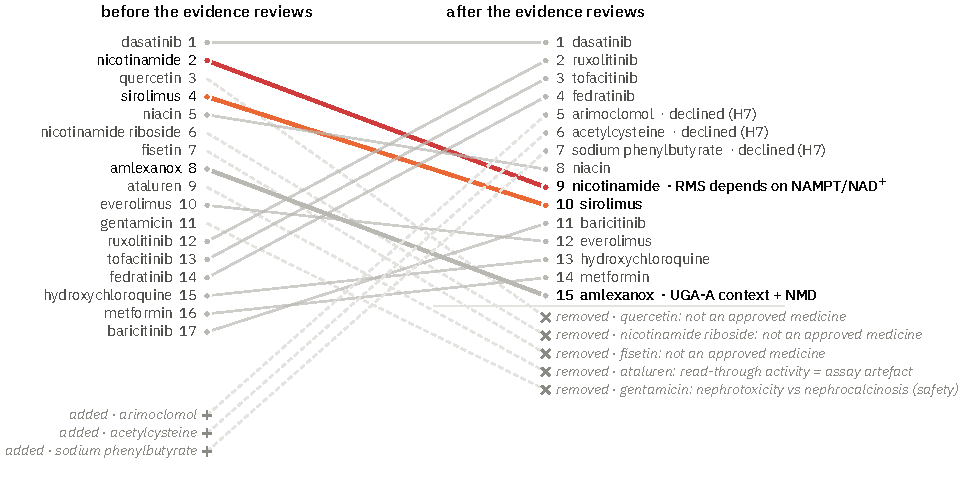
\includegraphics[width=\linewidth]{fig/t2_cambio.pdf}
\caption{How the evidence reviews changed the ranking. Left, ranks before (literature + connectivity); right,
after (approved medicines only). Nicotinamide fell because rhabdomyosarcoma depends on the pathway it feeds
(§\ref{sec:nad}); sirolimus rose on the first review and then fell again when its mouse evidence turned out to come
from monoallelic carriers (§\ref{sec:h3}); amlexanox fell when the read-through line was closed (§\ref{sec:rt});
five products were removed for regulatory status, efficacy or safety, and the proteostasis line was added and
declined.}
\label{fig:cambio}
\end{figure}

\subsection{Connectivity: what losing BUB1B does to a cell, and which drugs push the same way}
\label{sec:cmap}

\begin{figure}[htbp]
\centering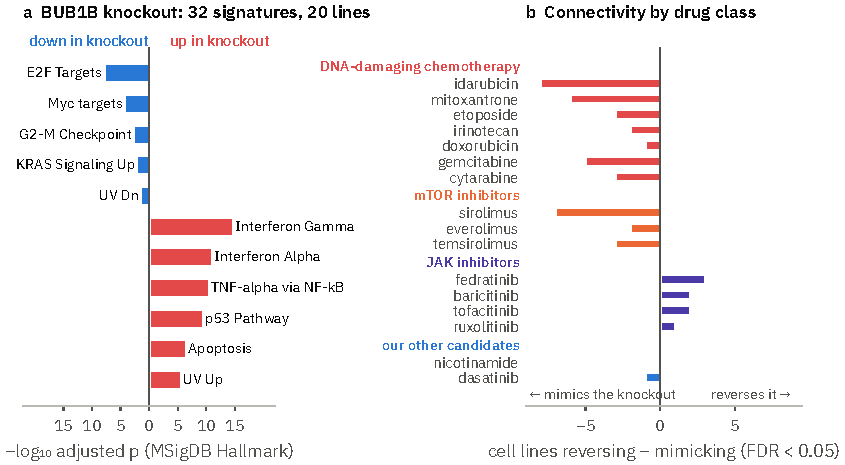
\includegraphics[width=\linewidth]{fig/t2_firma.pdf}
\caption{\textbf{a}, Hallmark pathways enriched among the 150 most up- and down-regulated genes of the consensus
\gene{BUB1B}-knockout signature (Enrichr). \textbf{b}, For selected drugs, number of cell lines in which the drug's
signature significantly reverses the knockout signature minus the number in which it mimics it.}
\label{fig:firma}
\end{figure}

\textbf{The signature.} Interferon-$\gamma$ and interferon-$\alpha$ responses, NF-$\kappa$B and p53 dominate the
up-regulated genes (top genes include \gene{CDKN1A}, \gene{ISG15}, \gene{IRF7}); E2F, MYC and G2–M programmes dominate
the down-regulated ones (Figure~\ref{fig:firma}a). This is the expected response to chromosome missegregation:
micronuclei sensed by cGAS–STING drive interferon signalling \citep{mackenzie,bakhoum}, p53 arrests the cycle, and
proliferation shuts down \citep{santaguida}.

\textbf{Validity check: mimickers.} The drugs that reproduce the signature in the most cell lines are dominated by
DNA-damaging or anti-proliferative chemotherapies (idarubicin 8 lines, mitoxantrone 7, gemcitabine, etoposide,
cytarabine, irinotecan), alongside other anti-proliferative agents such as sirolimus and bortezomib (8 lines each). A signature reproduced by genotoxic stress is biologically coherent, and it
supports the safety card directly: in a child whose cells already sit in this state, these agents are predicted to
add to it in normal tissue.

\textbf{Reversers, and how we actually used them.} 539 compounds reverse the signature significantly (FDR < 0.05)
in at least one cell line, and 25 do so in at least three net lines, so a ``top hit'' here means little on its own.
We did not pick H6 off the top of that list: the up-regulated arm is interferon-dominated, so we \emph{looked for}
JAK inhibitors in the reverser list and found four, three with no mimicking line and ruxolitinib with one, at ranks 15 (fedratinib), 38
(baricitinib), 43 (tofacitinib) and 154 (ruxolitinib). That is class consistency, not a data-driven discovery, and
we report it as such. There is no permutation control for how often a four-member drug class achieves this by
chance, which is the main reason H6 stays biomarker-gated at tier~4.

\textbf{What the top of the reverser list actually contains} is a better argument than the JAK inhibitors are. The
8th-ranked reverser is \textbf{tozasertib, an Aurora kinase inhibitor} --- a drug predicted to make this disease
worse, since it disables the same mitotic checkpoint machinery. The 24th is \textbf{EX-527, a SIRT1 inhibitor},
pointing against the very axis H1 is built on. Both reverse the knockout signature convincingly. This is the
cleanest demonstration we can offer that \textbf{reversing a transcriptional signature is not a therapeutic claim},
and it is why connectivity sits beside the score rather than inside it.

\textbf{Self-critique.} mTOR inhibitors consistently \textbf{mimic} the signature (sirolimus 8 lines, everolimus 3,
temsirolimus 3) because they deepen the anti-proliferative arm. We recorded this as contrary evidence for H3, one
of several reasons sirolimus now ranks tenth rather than first. The growth concern is partly allayed by 25
children on sirolimus without loss of linear growth \citep{hymes}, against one case report of growth failure
\citep{rangel}. \textit{Limits:} the signatures come from tumour cell lines after acute knockout, not from patient
cells with chronic partial deficiency; they are used for interpretation, safety and self-critique, not as evidence
of efficacy.

\subsection{Line-by-line rationale}

\begin{keybox}[title={S1 · Safety note (tier 0)}]
\begin{itemize}
\item \textit{Mechanism, in both directions.} Vinca alkaloids, taxanes and eribulin kill through
  checkpoint-dependent mitotic arrest. With low BUBR1 the prediction is genuinely two-sided: cells may slip out of
  arrest and survive with more missegregation (less tumour kill, more chromosomal damage in normal dividing tissue),
  or fail to sustain arrest and die faster (more sensitivity, more toxicity). Checkpoint-weakened cells are a
  classical setting for antimitotic \emph{hyper}sensitivity, so we present the ambiguity rather than resolve it.
  Either way the conclusion is closer monitoring, not avoidance.
\item \textit{Clinical signals in MVA.} Severe adverse reaction to dactinomycin in one biallelic \gene{BUB1B} child
  \citep{ochiai}; reduced-intensity chemotherapy for rhabdomyosarcoma in one PCS-MVA child \citep{nishitani};
  surveillance guidance for genomic-instability disorders \citep{nakano}; poor growth-hormone response in four MVA
  patients, none of them \gene{BUB1B} (§\ref{sec:casos}).
\item \textit{Organ-specific.} BubR1 insufficiency causes cardiac hypertrophy and fibrosis in mice
  (\pmid{40607964}), which supports cardiac monitoring with anthracyclines. BubR1-hypomorphic mice also show
  \emph{central} nervous system hypomyelination (\pmid{27922816}); peripheral nerves were not studied, so that paper
  does not by itself predict vincristine neuropathy, and we no longer claim it does.
\item \textit{The risk of the note itself is under-treatment.} This is the one deliverable most likely to be acted
  on, and the danger is that a flag against an antimitotic is read as a reason to de-escalate curative therapy. The
  note says so on its first line, recommends discussion and monitoring rather than substitution, and should be
  countersigned by a paediatric oncologist before use.
\item \textit{Deliverable.} A two-page pharmacogenomic note (\code{safety\_card.pdf}): section A for drugs the child
  may actually receive, section B for the paediatric label items of every candidate ranked here (dasatinib pleural
  effusion and bone growth; sirolimus proteinuria, troughs, CYP3A4 and live vaccines; JAK inhibitors zoster, TB and
  live vaccines; fedratinib's boxed warning for Wernicke's encephalopathy).
\end{itemize}
\end{keybox}

\textbf{H4 · Senescent cells (tier 1, as an experiment).}
\begin{itemize}
\item \textit{Evidence.} Genetic clearance of p16\textsuperscript{Ink4a}-positive cells delayed sarcopenia, cataract
  and lipodystrophy in BubR1-hypomorphic mice \citep{baker11}. It delayed onset and slowed progression; it did not
  rescue the phenotype and did not extend lifespan in that background.
\item \textit{Gap.} No senolytic drug has ever been tested in a BubR1 or aneuploidy model, which makes BubR1 H/L1002P
  mice \citep{sieben} the obvious and cheap experiment.
\item \textit{Contrary human evidence.} The best senolytic RCT (dasatinib + quercetin, 60 women) missed its primary
  endpoint \citep{farr}; the pulmonary fibrosis pilot did not change lung function \citep{justice}.
\item \textit{Connectivity, by the same standard as sirolimus.} Dasatinib reverses the knockout signature in 2 cell
  lines and mimics it in 3. We count mimicry against sirolimus, so it counts against dasatinib too: one more reason
  H4 is proposed as an experiment, not a treatment.
\item \textit{Caution.} Senescence has developmental roles, which argues for intermittent dosing and preclinical data
  first. Dasatinib has paediatric dosing and an oral suspension.
\end{itemize}

\textbf{H3 · mTORC1 (tier 3, low-dose sirolimus; tenth by score).}
\label{sec:h3}
\begin{itemize}
\item \textit{What the mouse study actually shows.} In the BubR1 allelic series \citep{sieben}, sarcopenia
  correlated with mTORC1 hyperactivity in mice carrying a \textbf{single} MVA allele. The biallelic genotype that
  mirrors this child --- truncating plus kinase-domain missense, X753/L1002P --- \textbf{died prematurely}; the
  viable biallelic model is H/L1002P, a hypomorph plus missense. No mTOR inhibitor was given in that study. An
  earlier draft of this report attributed the mTORC1 result to ``this child's allele class'', which was wrong; the
  correction costs H3 its strongest-looking support and is the main reason sirolimus fell from first to tenth. The child is alive where that mouse genotype was not; a
  mouse-to-human comparison of survival is too unreliable to say more than that p.Asn1002Lys \emph{might} retain
  more function than L1012P (§\ref{sec:alelo}).
\item \textit{Paediatric data, stated in full.} In ARST1431, temsirolimus added to VAC/VI in 297 children with
  intermediate-risk rhabdomyosarcoma gave \textbf{no event-free-survival benefit} (HR 0.86, 95\,\% CI 0.58--1.26,
  $p = 0.44$) and \textbf{more toxicity}: grade 3--4 anaemia in 58\,\% versus 41\,\%, and \textbf{one
  treatment-related death} in the temsirolimus arm \citep{gupta}. This is simultaneously the best paediatric
  feasibility evidence for an mTOR inhibitor in exactly this tumour and a serious caution in a child with a weak
  checkpoint and marrow exposure.
\item \textit{Drosophila, labelled honestly.} Feeding rapamycin to a fly model of MVA-like microcephaly partially
  rescued \textbf{neuroblast number} (the survival of aneuploid neuroblasts) \citep{milan} --- by our own taxonomy a \emph{tolerate}
  effect, not a correction --- and did not rescue progeny number or brain size.
\item \textit{A safety concern that needs its own caveat.} Rapamycin caused chromosome malsegregation and
  CREST-positive micronuclei in human lymphocytes and lymphoblasts \citep{bonatti}. It is a single 1998 in-vitro
  study, not replicated since, and its centrosome findings were in Chinese-hamster cells; set against it are
  decades of paediatric exposure in transplantation, tuberous sclerosis and vascular anomalies. We treat it as a
  reason to \textbf{monitor missegregation} (\%MN-RET, §\ref{sec:medir}) rather than as proof of harm.
\item \textit{If used.} Low, intermittent doses for muscle only, with phospho-S6, lean mass and growth endpoints,
  plus \%MN-RET as a safety readout and the label items in section B of the safety note.
\end{itemize}

\textbf{H1 · Raise BUBR1 abundance (tier 2, an NAD\textsuperscript{+} precursor, doubly gated).}
\begin{itemize}
\item \textit{Mechanism.} SIRT2 keeps BUBR1 Lys668 deacetylated, protecting it from degradation; falling
  NAD\textsuperscript{+} lowers BUBR1. SIRT2 overexpression extends the lifespan of BubR1-hypomorphic mice and the
  NAD\textsuperscript{+} precursor NMN raises BUBR1 in vivo \citep{north}. Lys668 lies upstream of codon 737, but the
  truncating allele's transcript is removed by NMD, so in practice the mark matters only on the missense allele's
  product.
\item \textit{Which precursor, and a problem with the obvious one.} The tested modality is NMN, which is not an
  approved medicine. Of the approved precursors, \textbf{nicotinamide is itself a non-competitive sirtuin inhibitor
  at physiological concentrations} \citep{bitterman} --- it is the reaction product of the deacetylation this line
  depends on. \textbf{Niacin}, which enters via the Preiss--Handler route, carries no such objection and is the
  better mechanistic match; we score nicotinamide 0.2 lower on fit for this reason. That the two still finish level
  is a reminder that the score is a summary, not an argument.
\item \textit{Fit, and its condition.} The line exists only if the missense allele belongs to the low-abundance
  class, which is unmeasured but likely (prior 0.75, §\ref{sec:alelo}), giving $M = 0.8 \times 0.75 = 0.6$ before
  the per-drug adjustment. Nicotinamide has a large paediatric safety record \citep{gale,knip}.
\item \textit{Contrary evidence.} SIRT2 does not extend lifespan in wild-type mice \citep{wu}; and, decisively for
  timing, rhabdomyosarcoma depends on NAMPT (§\ref{sec:nad}).
\item \textit{Why this is tier 2 and not tier 4.} Both of its blockers are \emph{measurable facts about this child},
  not gaps in the literature: the allele class (one immunoblot) and remission status (already known to the treating
  team). Establish both and this line ranks first overall (§\ref{sec:ejes}) --- which is why the report's main
  recommendation is a measurement.
\end{itemize}

\textbf{H6 · Interferon / JAK–STAT (tier 4, biomarker-gated).}
\begin{itemize}
\item \textit{Rationale.} The up-regulated arm of the knockout signature is interferon-dominated; the four JAK inhibitors
  in LINCS reverse it as a class, though none near the top (§\ref{sec:cmap}); and JAK inhibition reduces the SASP
  and frailty in old mice \citep{xu}.
\item \textit{Human target confirmation, and its limit.} A 2024 narrative review reports a chronic immune response
  in MVA patients \citep{malumbres}. \textbf{No interferon signature has been published for any MVA patient}: the
  target is plausible, not confirmed, which is why this line is gated on measuring it in the child.
\item \textit{Paediatric precedent.} Baricitinib in children with interferonopathies, given under a compassionate-use
  protocol (\nct{NCT01724580}) \citep{sanchez}. Two later paediatric baricitinib or JAK-inhibitor studies in the same
  diseases, not part of that paper: \nct{NCT04517253} (Japan; terminated) and \nct{NCT03921554} (Aicardi--Goutières;
  completed).
\item \textit{Decisive caveat.} The inflammatory signal of aneuploid cells drives their immune clearance
  \citep{santaguida}; blocking it could weaken tumour immunosurveillance. Not proposed for chemoprevention.
\end{itemize}

\textbf{H5 · Aneuploid-selective stress (not pursued; one member is an anti-target here).}
\label{sec:h5}
AICAR, 17-AAG and chloroquine selectively impair aneuploid cells \citep{tang}; metformin and hydroxychloroquine
are approved proxies. The evidence is from cells only, and in a mosaic child these drugs could also deplete normal
tissue. One of the three, however, turns out to be an \textbf{anti-target for this particular genotype}: 17-AAG
acts on HSP90, and HSP90 is the chaperone that folds kinase-domain BUBR1 missense mutants --- inhibiting it
removes essentially all of the mutant protein while barely touching wild type, and blocking the proteasome
prevents that loss \citep{suij}. A drug chosen from the downstream phenotype would here destroy the residual
protein the child depends on, if scenario~A holds. The objection concerns 17-AAG, not the approved proxies, so it does not
lower this line's evidence score; instead HSP90 inhibitors are added pre-emptively to the safety card.

\textbf{H7 · Proteostasis amplification and antioxidants (considered, declined).}
\label{sec:h7}
This is a commonly proposed alternative for this genotype, so we evaluated it rather than passing over it in
silence.
\begin{itemize}
\item \textit{The lever is real.} Mutant BUBR1 stability depends on HSP90 and on escape from the proteasome
  \citep{suij}, and aneuploid human cells are impaired in HSP90-dependent folding with a compromised heat-shock
  response, so raising HSF1 restores HSP90 expression and folding in exactly the cell state this child has
  \citep{donnelly}. Arimoclomol amplifies that response and is an approved medicine with paediatric experience
  (Niemann-Pick C, with miglustat; \citealp{mengel}); sodium phenylbutyrate is a chemical-chaperone comparator.
\item \textit{The objection comes from the same paper that validates the lever.} \citet{donnelly} identify HSF1
  overexpression as the \textbf{first described aneuploidy-\emph{tolerating} event in human cells}: its effect is
  to make chromosomally abnormal cells viable. In a child with a cancer-predisposition syndrome and a history of
  rhabdomyosarcoma, a mechanism whose benefit is inseparable from the survival of chromosomally abnormal cells is
  on the wrong side of the trade-off. The same logic applies to the antioxidant arm, which accelerates tumour
  progression and metastasis in mouse models \citep{sayin,wiel}.
\item \textit{Where it would reopen.} Only if rung~1 confirms scenario~A \emph{and} an assay separates BUBR1
  restoration from general survival of aneuploid cells --- concretely, micronuclei must fall, not merely cell
  number rise. That is a falsifiable condition, not a polite refusal.
\end{itemize}

\subsection{A conflict at the heart of our initial lead: NAD\textsuperscript{+} and rhabdomyosarcoma}
\label{sec:nad}
\begin{cautionbox}[title={What we found}]
Rhabdomyosarcoma, the tumour in this child's history (remission status to be documented), depends on \textbf{NAMPT}, the rate-limiting enzyme of the
NAD\textsuperscript{+} salvage pathway. The clinical NAMPT inhibitor OT-82 depleted NAD\textsuperscript{+} and
inhibited growth at $\leq$1~nmol/L in all ten molecularly diverse RMS cell lines, and produced complete tumour
regression in orthotopic models \citep{mckay}. Nicotinamide is the direct substrate of NAMPT; nicotinamide riboside
bypasses NAMPT but still raises the NAD\textsuperscript{+} pool. NR supplementation also increased cancer prevalence and
brain metastases in a breast-cancer model \citep{maric}.
\end{cautionbox}
Against this, the ONTRAC phase 3 trial found that nicotinamide \textit{reduced} new non-melanoma skin cancers by 23\,\%
in 386 high-risk adults \citep{ontrac}. That benefit is attributed to repair of UV-induced DNA damage, biology that does
not transfer to a NAMPT-dependent sarcoma: ONTRAC supports tolerability, not oncological safety here. We
\textbf{condition rather than delete} the line:
\begin{enumerate}
\item BUBR1 stabilisation is chronic and preventive; NAMPT dependency is an acute need of an existing tumour.
\item No NAD\textsuperscript{+} precursor unless the child is in documented remission, with intensified surveillance
  \citep{nakano} as a stopping rule.
\item The first experiment must show that an NAD\textsuperscript{+} precursor (niacin) raises BUBR1 in this child's own cells; if it does not, the
  risk is not worth taking.
\item On the safety card: if the tumour recurs, a NAMPT inhibitor would be a rational agent and a
  NAD\textsuperscript{+} supplement would be expected to antagonise it.
\item Precedent for caution rather than prohibition: a completed n-of-1 study of NR in Li-Fraumeni syndrome, another
  cancer-predisposition syndrome (\nct{NCT03789175}).
\end{enumerate}
No selective SIRT2 activator exists (the published chemical matter is inhibitors), so the trade-off cannot currently be
engineered away.

\subsection{Closing the read-through line on allele-specific evidence}
\label{sec:rt}
Read-through efficiency depends mainly on the stop codon and its +4 nucleotide, with the preference C > U > A/G
\citep{mangk}. We computed the context of this allele from the public reference CDS (\code{contexto\_stop.py};
Figure~\ref{fig:codon}).

\begin{figure}[htbp]
\centering
\begin{tikzpicture}[font=\sffamily\small, b/.style={minimum width=6.2mm, minimum height=6.2mm, inner sep=0pt, rounded corners=1.5pt, text=white, font=\sffamily\bfseries\small}]
  \node[anchor=east, text=ink2] at (-0.3,0.9) {reference};
  \node[anchor=east, text=ink2] at (-0.3,-0.2) {variant};
  \foreach \i/\l/\c in {0/C/brand,1/C/brand,2/A/aqua,4/G/accent,5/A/aqua,6/G/accent,8/T/violet,9/T/violet,10/A/aqua,12/A/aqua,13/G/accent,14/T/violet,16/G/accent,17/C/brand,18/C/brand}
    \node[b, fill=\c] at (\i*0.66,0.9) {\l};
  \foreach \i/\l/\c in {0/C/brand,1/C/brand,2/A/aqua,4/G/accent,5/A/aqua,6/G/accent,8/T/violet,9/G/accent,10/A/aqua,12/A/aqua,13/G/accent,14/T/violet,16/G/accent,17/C/brand,18/C/brand}
    \node[b, fill=\c] at (\i*0.66,-0.2) {\l};
  \draw[critical, line width=1pt, rounded corners=2pt] (5.0,-0.62) rectangle (7.05,0.22);
  \node[font=\sffamily\scriptsize\bfseries, text=critical, below] at (6.03,-0.62) {UGA stop · favourable};
  \draw[critical, line width=1.2pt, rounded corners=2pt, dashed] (7.55,-0.62) rectangle (8.3,0.22);
  \node[font=\sffamily\scriptsize\bfseries, text=critical, below, align=center] at (8.6,-0.62) {+4 = A\\unfavourable};
  \node[font=\sffamily\scriptsize, text=ink2] at (6.6,1.55) {Leu737 (TTA)};
  \draw[-{Stealth}, ink2] (5.94,0.55) -- (5.94,0.25);
  \node[draw=rule, fill=panel, rounded corners=2pt, align=left, font=\sffamily\scriptsize, anchor=north west, text width=9.5cm] at (-2.0,-1.75)
    {\textbf{Context UGA-A}\enspace stop identity: most permissive \textcolor{good}{$\checkmark$}\enspace·\enspace +4 base: weakest group (C>U>A/G) \textcolor{critical}{$\times$}\enspace·\enspace 314 codons left \arr\ NMD \textcolor{critical}{$\times$}\enspace\arr\enspace\textbf{\textcolor{critical}{line closed (current evidence)}}};
\end{tikzpicture}
\caption{The allele-level argument. Reference and variant coding sequence around codon 737 (codons separated). The
stop codon is the most read-through-permissive kind, but the base that follows it is in the least favourable group,
and the transcript is expected to undergo nonsense-mediated decay.}
\label{fig:codon}
\end{figure}

This is a two-feature reading of the context (stop identity and +4 base); \citet{mangk} also publish a predictor
trained on the extended context, which we did not run. Combined with drug-level evidence, it closes the line
\emph{on current evidence}:
\begin{itemize}
\item \textbf{Ataluren removed}: its read-through activity is attributed to an off-target luciferase artefact
  \citep{mcelroy}; the cystic fibrosis phase 3 failed and EMA did not renew its conditional authorisation.
\item \textbf{Amlexanox demoted}: its original report showed more nonsense-containing mRNA and full-length protein
  (\pmid{22938201}), but independent controlled comparisons did not reproduce the mRNA increase (\pmid{33396210},
  \pmid{37866515}); its proposed action is NMD-related rather than read-through.
\item \textbf{The compounds that correct UGA alleles are not approved}: 2,6-diaminopurine \citep{trzaska}, G418 and
  SMG1 inhibitors, several of them toxic; the approved aminoglycoside gentamicin reads through only weakly and is
  nephrotoxic, a poor fit for a child with nephrocalcinosis.
\end{itemize}
The recommendation is an experiment, not a drug: a non-luciferase reporter carrying the native UGA-A context, with and
without NMD inhibition, in patient-derived cells.

\subsection{What has actually been given to people with MVA}
\label{sec:casos}
We screened \textbf{every PubMed record on MVA or premature chromatid separation} (132 records;
\code{revision\_casos.py}) for treatment terms and read every hit. Only 9 mention any treatment, and none reports a
disease-modifying drug.
\begin{table}[H]\tablefont
\begin{tabularx}{\linewidth}{@{}P{4.4cm}P{2.3cm}LP{1.9cm}@{}}
\toprule\thead{Exposure} & \thead{MVA type} & \thead{What happened} & \thead{Source}\\\midrule
Dactinomycin for Wilms tumour & MVA1 (\gene{BUB1B}) & severe adverse reaction prevented further chemotherapy & \pmid{31081598}\\
Chemotherapy for rhabdomyosarcoma & PCS-MVA & reduced-intensity chemotherapy & \pmid{31184400}\\
Chemoradiotherapy \emph{advised}, orbital embryonal RMS after Wilms & MVA3 (\gene{TRIP13}) & second malignancy; treatment recommended, but neither its delivery nor any outcome is reported & \pmid{42595739}\\
Stem cell transplant (reduced-intensity conditioning) for MDS with monosomy 7 & MVA1 (\gene{BUB1B}) & tolerated, haematological recovery, then graft rejection and fatal sepsis & \pmid{31053147}\\
Growth hormone for short stature & MVA2 (\gene{CEP57}) ×3, MVA ×1 & poor or no response in all four; possible growth-plate resistance & \pmid{35434947} and 3 others\\\bottomrule
\end{tabularx}\end{table}
Two conclusions feed the safety card. Growth hormone combines low expected benefit with a cancer-predisposition
concern. Cytotoxic therapy is poorly tolerated in MVA1, and reduced-intensity regimens are already the published
practice.

\section{How we would know whether it works in this child}
\label{sec:medir}

Every repurposing report, including the earlier drafts of this one, ends at ``it should be tested''. For a disease
with fewer than 50 known patients that is where the real problem starts, because the usual endpoints do not work:
tumour incidence needs decades and a cohort, and a lymphocyte karyotype reports an aneuploidy burden accumulated
over years, so it cannot tell whether a drug started last month is helping. What is missing is an endpoint that
moves in weeks.

\begin{keybox}[title={The endpoint: micronucleated reticulocytes (\%MN-RET)}]
\tablefont
\begin{tabularx}{\linewidth}{@{}P{2.9cm}L@{}}
\textbf{What it counts} & micronuclei --- fragments left outside the nucleus by a missegregation event. It is the direct product of this disease's defect, not a proxy for it\\
\textbf{Why reticulocytes} & they circulate for 1--2 days, so the measurement is a \textbf{recent error rate}, not a lifetime accumulation. The spleen removes micronucleated erythrocytes, which is why the mature red-cell assay fails in humans and the reticulocyte one works\\
\textbf{How} & one blood draw; flow cytometry scores $\geq$20{,}000 CD71\textsuperscript{+} reticulocytes per sample \citep{dertinger,dertinger11}\\
\textbf{Paediatric reference} & upper bound of the 90\,\% tolerance interval in paediatric controls = \textbf{0.42\,\%} \citep{baig}\\
\textbf{Status in MVA} & \textbf{never measured}. This is rung~0, and it is worth doing whether or not any drug is ever given: the first result is diagnostic in the sense of a disease-activity observation (not yet a validated diagnostic
test) --- whether this disease is visibly active in blood, and how much --- and it applies to every MVA patient, not only this one\\
\textbf{Two-way information} & it falls if a drug reduces missegregation and \textbf{rises if a drug adds it} --- which is why it gates sirolimus, once our top-scoring candidate (§\ref{sec:h3})
\end{tabularx}
\end{keybox}

\textbf{The design, and what it can actually resolve.} We simulated an n-of-1 trial on this endpoint
(\code{scripts/t2/nof1.py}; public parameters only). Alternating on/off blocks; with 20,000 CD71\textsuperscript{+}
reticulocytes per sample the expected count is in the hundreds, so $\log(y/N)$ is near-normal. \textbf{The
between-visit variability $\sigma$ is not assumed known} --- it is estimated from the same data, so the posterior
for the log rate ratio is a Student $t$ with $n-2$ degrees of freedom. An earlier version conditioned on the true
$\sigma$, which inflated power and understated false positives for a quantity the report itself says has never been
measured. Every cell uses common random numbers and carries its Monte Carlo standard error.

\begin{figure}[htbp]
\centering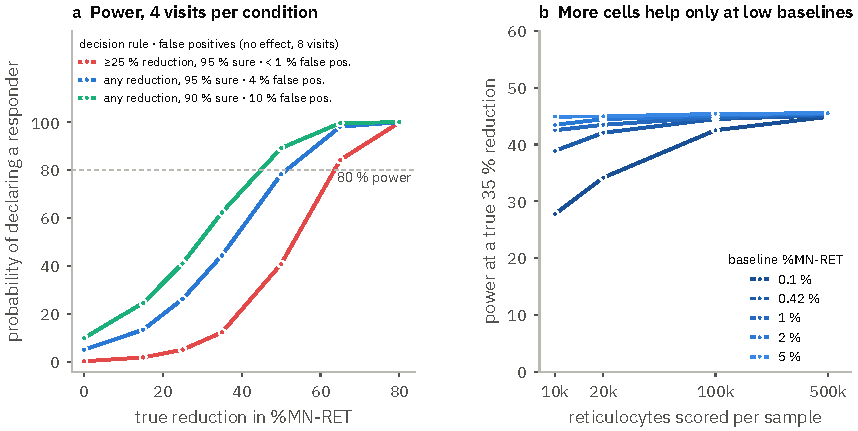
\includegraphics[width=\linewidth]{fig/t2_nof1.pdf}
\caption{\textbf{a}, Power against the true reduction in \%MN-RET for three candidate responder rules, with four
on/off visits per condition, $\sigma = 0.35$, 20,000 reticulocytes per sample and an assumed 2\,\% baseline; each
rule is labelled with its own false-positive rate. \textbf{b}, Power at a true 35\,\% reduction by baseline and by
cells scored: counting more cells buys almost nothing except at baselines near or below the paediatric reference.}
\label{fig:nof1}
\end{figure}

Three results, and the first is unwelcome:

\begin{enumerate}
\item \textbf{The strict rule is too strict to be useful.} Requiring $P(\text{reduction} \geq 25\,\%) \geq 95\,\%$
  detects only a \textbf{63\,\% or larger} true reduction at 80\,\% power with four visits per condition; a 35\,\%
  reduction is caught 12\,\% of the time. Its false-positive rate is under 1\,\%, far below the conventional 5\,\%,
  which is the price being paid. The conventional rule --- any reduction with 95\,\% posterior certainty --- is
  calibrated at the advertised rate and needs a 51\,\% reduction, or 9 visits per condition to reach a 35\,\% one.
  Proposing this endpoint without the power calculation would be proposing an experiment that cannot answer its own
  question.
\item \textbf{Counting more cells helps only if the baseline is low.} At the assumed 2\,\% baseline, going from
  10,000 to 500,000 reticulocytes per sample moves power from 43.5\,\% to 45.5\,\%, because the counting term $1/y$
  is negligible beside $\sigma^2 = 0.12$. At a baseline of 0.1\,\% --- below the paediatric reference ceiling --- the
  same change moves it from 27.8\,\% to 44.9\,\%. So the rule is conditional, and rung~0 establishes which regime
  applies: \emph{if the baseline exceeds about 1\,\%, spend the budget on repeated visits rather than deeper runs.}
\item \textbf{The decision rule dominates every other knob.} Power at a 35\,\% reduction ranges from 12\,\% under
  the strict rule to 62\,\% under ``any reduction, 90\,\% certainty'', whose false-positive rate is 10\,\%. That
  trade-off --- not the power figure alone --- is what a clinical team and a family have to choose between, and the
  right time to choose is before the first sample.
\end{enumerate}

\noindent Every number above is conditional on $\sigma$, the between-visit variability, which has never been
measured in anyone with MVA. \textbf{So the first study is not a drug study}: establish the baseline and $\sigma$
in this child with repeated sampling off treatment. That single measurement also tests the disease model --- a
\%MN-RET within the paediatric reference range would be evidence against the disease model on which the
measurement-led part of this report rests, and
we would rather find that out from a blood draw than from a failed treatment. \textbf{A ready-to-use one-page
protocol} for that study (\code{reports/t2/rung0\_protocol.pdf}) specifies the samples, the confounders to record
(infection and malnutrition raise \%MN-RET in children; cytotoxic therapy raises it up to 26-fold, peaking 3--5 days after starting),
the pre-declared decision table, and how many on/off visits each responder rule needs for the $\sigma$ that the
child turns out to have.

\section{How a medicine like this gets validated}
\label{sec:validacion}
No clinical trial for MVA is registered anywhere (ClinicalTrials.gov, October 2026). With fewer than 50 known
patients a randomised trial is impossible, but comparable diseases have walked a route with four rungs
(Figure~\ref{fig:escalera}).

\begin{figure}[htbp]
\centering
\begin{tikzpicture}[font=\sffamily\scriptsize,
  step/.style={draw=#1, line width=0.8pt, fill=#1!6, rounded corners=2pt, align=left, inner sep=4pt, text width=3.25cm, minimum height=1.55cm, anchor=south west},
  pre/.style={align=left, inner sep=1pt, text width=3.25cm, anchor=north west, font=\sffamily\scriptsize\itshape, text=ink2},
  fl/.style={-{Stealth[length=2mm]}, draw=good, line width=0.8pt}]
  \foreach \i/\c/\t/\r/\p in {
    0/brand/{1 · Patient's own cells}/{\textbf{BUBR1 level $\pm$ CHX chase $\rightarrow$ allele scenario A or B}; time in mitosis, \% aneuploid cells, micronuclei}/{gates every restorative line},
    1/violet/{2 · Tissue model}/{iPSC-derived myotubes: mTORC1 activity, senescence, SASP}/{standard translational step},
    2/aqua/{3 · Existing mouse model}/{BubR1 H/L1002P, matching allele classes: lifespan, sarcopenia, tumours}/{no senolytic ever tested in it},
    3/accent/{4 · n-of-1 protocol}/{pre-declared responder criteria; on/off blocks; natural-history control}/{precedents: lonafarnib (progeria), sirolimus (Castleman)}}{
    \node[step=\c] (s\i) at (\i*4.15,\i*0.42) {\textbf{\t}\\[2pt]\r};
    \node[pre] at ([yshift=-1.5mm]s\i.south west) {\p};
  }
  \foreach \i/\j in {0/1,1/2,2/3} \draw[fl] (s\i.east) -- node[above, font=\sffamily\scriptsize\bfseries, text=good, sloped]{go} (s\j.west);
\end{tikzpicture}
\caption{The validation ladder. Each rung has a go / no-go readout. Preceding all of them is \textbf{rung 0}
(§\ref{sec:medir}): measure \%MN-RET and its between-visit variability in this child, off treatment --- it costs a
blood draw, it is the only endpoint that moves in weeks, and it can falsify the disease model before anyone is
exposed to anything. Rung~1 then decides the allele scenario, and with it whether any restorative line exists.}
\label{fig:escalera}
\end{figure}

\textbf{Making one patient's treatment into evidence.} Define the responder in advance (a common weakness of published
n-of-1 trials); use the patient as their own control with on/off blocks and Bayesian analysis for reversible
endpoints; and use natural history as an external control for endpoints that cannot be switched off. Progeria shows
this works: lonafarnib was approved on a single-arm cohort compared with untreated natural-history controls, with
mortality 3.7\,\% vs 33.3\,\% \citep{gordon}. The closest precedent to this project is \textbf{sirolimus in idiopathic
multicentric Castleman disease} \citep{fajgenbaum}: a pathway measured in the patients themselves, an approved drug
repurposed against it, remission, then a prospective trial (\nct{NCT03933904}). Our pipeline applies the same logic one
step earlier.

\textbf{Regulatory routes} (checked against primary texts; the patient's jurisdiction is not known to us).
\begin{table}[H]\tablefont
\begin{tabularx}{\linewidth}{@{}P{3.3cm}LL@{}}
\toprule\thead{Situation} & \thead{United States} & \thead{European Union}\\\midrule
Physician prescribes an approved drug off-label & outside FDA's IND rules: ``this part does not apply to the use in the practice of medicine for an unlabeled indication'' (21 CFR 312.2(d)) & regulated nationally; typically the physician decides, documents the justification, obtains informed consent and follows the centre's protocol, usually with no case-by-case agency authorisation (in the EU, under each member state's rules on medicines in
special situations)\\
Structured n-of-1 study of an approved drug & may be IND-exempt if 21 CFR 312.2(b)(1)(i)–(v) hold (no labelling claim, IRB, consent); condition (iii) on risk in a special population needs FDA discussion & can qualify as a \textbf{low-intervention clinical trial} (Reg. (EU) 536/2014, art.~2(2)(3)): authorised medicine used in an evidence-based way, minimal added risk\\
Expanded access / compassionate use & Form FDA 3926; for \textit{investigational} drugs only & Art.~83 Reg. (EC) 726/2004; for \textit{unauthorised} medicines only\\\bottomrule
\end{tabularx}\end{table}
In both frameworks the barrier to trying a ranked candidate is clinical and ethical, not regulatory, and both expect
documented target engagement, which the first rung supplies. Sirolimus, everolimus, dasatinib and tofacitinib all
exist in oral liquid or dispersible forms that can be dosed by weight in a child.

\textbf{What we would do first:} (0) \%MN-RET and its variability in this child, off treatment, which costs a blood
draw and sets up everything else; (1) patient cells, to decide the allele scenario and so gate H1 and H7;
(2) BubR1 H/L1002P mice with three arms (vehicle, dasatinib, dasatinib + quercetin), as the gate for H4; (3) a
non-luciferase read-through reporter, as the reopening condition for H2; (4) only then, and only in remission, an
n-of-1 protocol with the clinical team, with the responder rule agreed in advance.

\section{Scalability}
\begin{itemize}
\item \textbf{New patient or gene:} a new \code{hipotesis.yaml}; \code{cmap.py}, \code{revision\_casos.py},
  \code{contexto\_stop.py} and \code{estructura.py} all take a gene or a change as a parameter.
\item \textbf{Tested, not just claimed:} re-running connectivity for the other MVA and checkpoint genes
  (\code{cmap.py --comparar}) showed that CEP57, TRIP13, BUB3 and MAD2L1 have \textbf{no knockout signatures in LINCS},
  so for them the pipeline runs on literature and labels only. BUB1 and TTK are profiled; their signatures correlate
  weakly with BUB1B's (Spearman $\rho$ 0.06 and 0.27), sharing the proliferation and p53 response but not the leading
  interferon programme. H6 is therefore supported for BUB1B specifically, and the pipeline reports where a data
  source does not exist instead of filling the gap.
\item \textbf{Staying current and cheap:} ChEMBL target expansion can add newly approved drugs automatically (in this
  run it added none; see the limitations); label mining
  keeps safety current; all sources are public and a full run takes minutes on a laptop.
\end{itemize}

\section{Limitations}
\begin{itemize}
\item Efficacy evidence is preclinical; no drug has been tested in MVA patients.
\item \textbf{The class of the missense allele is unmeasured} (§\ref{sec:alelo}). The 0.75/0.25 prior is a
  judgement calibrated on one study, and under scenario~B two of our seven lines do not exist.
\item \textbf{The ranking is sensitive to two curated inputs for H1}, and we publish the counterfactual rather than
  claim robustness (§\ref{sec:ejes}). More generally, every mechanistic-fit value is an expert judgement; they are
  exposed in the YAML and stress-tested over $\pm$0.30, with safety over $\pm$0.15.
\item \textbf{The evidence term still depends on curation depth.} Contrary studies are now weighted by level and
  capped, and harms moved to safety, but a line we interrogated harder can still score lower than one we did not.
  The per-line table in \code{candidatos.md} reports how many items of each kind we curated, so the asymmetry is
  visible.
\item \textbf{Every ranked drug was hand-seeded.} The automated ChEMBL target expansion contributed no new drug
  here --- mechanism annotation for spindle-checkpoint biology is too sparse --- so the composition of the candidate
  list is ours, which is why axis conclusions are reported per line rather than averaged over drugs.
\item \textbf{The power calculation rests on an assumed \%MN-RET baseline and variability} that have never been
  measured in MVA. $\sigma$ is now estimated from the data rather than assumed known, and every figure carries its
  Monte Carlo error, but the absolute numbers are conditional on the baseline rung~0 will establish.
\item The three therapeutic axes are a deliberate simplification: a real drug can act on more than one, which is
  exactly why H7 is recorded with a primary and a risk axis rather than a single label.
\item Connectivity signatures come from tumour cell lines after acute knockout, and we have no permutation control
  for how often a drug class reverses the signature by chance (§\ref{sec:cmap}).
\item Label mining is keyword-based and US-centric; flags were reviewed manually. No dosing, drug--drug interaction
  or formulation-stability analysis was performed.
\item The case-literature screen covers titles and abstracts (122 of 132 records have one), so details in full
  texts may be missed.
\item Senescent-cell burden has never been measured in MVA patients.
\item Regulatory routes are summarised for orientation, not as legal advice.
\end{itemize}

\section{Data protection and LLM use}
\begin{itemize}
\item \textbf{LLM declaration} (organisers' format, discussion \#2): \textit{Anthropic Claude via the Claude Code CLI,
  Claude Max (consumer tier), model-training opt-out enabled (``Help improve Claude'' off), no feedback provided on any
  output, no content flagged for safety review.} Opted-out conversations are not used for training and are retained
  for 30 days.
\item LLM sub-agents assisted the literature screening. \textbf{Every citation was then verified against PubMed,
  ClinicalTrials.gov or the primary regulatory text}; one misattributed first author was corrected, and claims that
  could not be verified are not cited.
\item Track~2 used only gene-, pathway- and drug-level information. The one sequence-level analysis (§\ref{sec:rt})
  used the public reference CDS and the already-submitted coding change.
\end{itemize}

\needspace{9\baselineskip}
\section*{Acknowledgement}
This work was made possible through the Hackathon, organized by Sage Bionetworks in partnership with the MVA Society,
Hugging Face, and BEACON (The Benchmarking, Evaluation, and Assessment Consortium for Science), with prize sponsorship
from AWS and Anthropic. We are deeply grateful to the child and their family who generously contributed their data
and their story to advance research into this rare disease. We acknowledge their trust in making this Hackathon
possible.

\section*{References}
\begin{refs}
\item Baig A et al. Assessment of systemic genetic damage in pediatric inflammatory bowel disease. \textit{Environ Mol Mutagen} 2020. \pmid{32761646}.
\item Baker DJ et al. BubR1 insufficiency causes early onset of aging-associated phenotypes and infertility in mice. \textit{Nat Genet} 2004. \pmid{15208629}.
\item Baker DJ et al. Clearance of p16Ink4a-positive senescent cells delays ageing-associated disorders. \textit{Nature} 2011. \pmid{22048312}.
\item Baker DJ et al. Increased expression of BubR1 protects against aneuploidy and cancer and extends healthy lifespan. \textit{Nat Cell Biol} 2013. \pmid{23242215}.
\item Bakhoum SF et al. Chromosomal instability drives metastasis through a cytosolic DNA response. \textit{Nature} 2018. \pmid{29342134}.
\item Bitterman KJ et al. Inhibition of silencing and accelerated aging by nicotinamide, a putative negative regulator of yeast Sir2 and human SIRT1. \textit{J Biol Chem} 2002. \pmid{12297502}.
\item Bohers E et al. Gradual reduction of BUBR1 protein levels results in premature sister-chromatid separation then in aneuploidy. \textit{Hum Genet} 2008. \pmid{18932004}.
\item Bonatti S et al. Inhibition of the Mr 70,000 S6 kinase pathway by rapamycin results in chromosome malsegregation in yeast and mammalian cells. \textit{Chromosoma} 1998. \pmid{9914383}.
\item Chen AC et al. A phase 3 randomized trial of nicotinamide for skin-cancer chemoprevention (ONTRAC). \textit{N Engl J Med} 2015. \pmid{26488693}.
\item Choi CI et al. The progeroid gene BubR1 regulates axon myelination and motor function. \textit{Aging (Albany NY)} 2016. \pmid{27922816}.
\item Dertinger SD et al. Micronucleated CD71-positive reticulocytes: a blood-based endpoint of cytogenetic damage in humans. \textit{Mutat Res} 2003. \pmid{14644356}.
\item Dertinger SD et al. Flow cytometric scoring of micronucleated erythrocytes: an efficient platform for assessing in vivo cytogenetic damage. \textit{Mutagenesis} 2011. \pmid{21164195}.
\item Donnelly N et al. HSF1 deficiency and impaired HSP90-dependent protein folding are hallmarks of aneuploid human cells. \textit{EMBO J} 2014. \pmid{25205676}.
\item Fajgenbaum DC et al. Identifying and targeting pathogenic PI3K/AKT/mTOR signaling in IL-6-blockade-refractory idiopathic multicentric Castleman disease. \textit{J Clin Invest} 2019. \pmid{31408438}.
\item Farr JN et al. Effects of intermittent senolytic therapy on bone metabolism in postmenopausal women: a phase 2 randomized controlled trial. \textit{Nat Med} 2024. \pmid{38956196}.
\item Feng B et al. A novel CEP57 variant associated with mosaic variegated aneuploidy syndrome in a Chinese female. \textit{Mol Genet Genomic Med} 2022. \pmid{35434947}.
\item Gale EA et al. European Nicotinamide Diabetes Intervention Trial (ENDIT). \textit{Lancet} 2004. \pmid{15043959}.
\item González-Blanco A et al. Proteostasis failure and mitochondrial dysfunction contribute to chromosomal instability-induced microcephaly. \textit{Nat Commun} 2026. \pmid{41820377}.
\item Gordon LB et al. Association of lonafarnib treatment vs no treatment with mortality rate in Hutchinson-Gilford progeria syndrome. \textit{JAMA} 2018. \pmid{29710166}.
\item Gupta AA et al. Addition of temsirolimus to chemotherapy in intermediate-risk rhabdomyosarcoma (ARST1431). \textit{Lancet Oncol} 2024. \pmid{38936378}.
\item Hymes LC, Warshaw BL. Linear growth in pediatric renal transplant recipients receiving sirolimus. \textit{Pediatr Transplant} 2011. \pmid{21884345}.
\item Justice JN et al. Senolytics in idiopathic pulmonary fibrosis: first-in-human, open-label pilot. \textit{EBioMedicine} 2019. \pmid{30616998}.
\item Knip M et al. Safety of high-dose nicotinamide: a review. \textit{Diabetologia} 2000. \pmid{11126400}.
\item Laberko A et al. Hematopoietic stem cell transplantation in a patient with type 1 mosaic variegated aneuploidy syndrome. \textit{Orphanet J Rare Dis} 2019. \pmid{31053147}.
\item Mackenzie KJ et al. cGAS surveillance of micronuclei links genome instability to innate immunity. \textit{Nature} 2017. \pmid{28738408}.
\item Malumbres M. Mosaic variegated aneuploidy in development, ageing and cancer. \textit{Nat Rev Genet} 2024. \pmid{39169218}.
\item Mangkalaphiban K et al. Extended stop codon context predicts nonsense codon readthrough efficiency in human cells. \textit{Nat Commun} 2024. \pmid{38509072}.
\item Maric T et al. A bioluminescent probe for nicotinamide riboside uptake reveals a link between metastasis and NAD+ metabolism. \textit{Biosens Bioelectron} 2023. \pmid{36371959}.
\item McElroy SP et al. A lack of premature termination codon read-through efficacy of PTC124 (ataluren). \textit{PLoS Biol} 2013. \pmid{23824517}.
\item McKay-Corkum GB et al. Inhibition of NAD+-dependent metabolic processes induces cellular necrosis and tumor regression in rhabdomyosarcoma models. \textit{Clin Cancer Res} 2023. \pmid{37616468}.
\item Mengel E et al. Efficacy and safety of arimoclomol in Niemann-Pick disease type C: results from a double-blind, randomised, placebo-controlled trial. \textit{J Inherit Metab Dis} 2021. \pmid{34418116}.
\item Nakano Y et al. Update on recommendations for cancer screening and surveillance in children with genomic instability disorders. \textit{Clin Cancer Res} 2024. \pmid{39264246}.
\item Nishitani-Isa M et al. Rhabdomyosarcoma with premature chromatid separation–mosaic variegated aneuploidy syndrome: reduced-intensity chemotherapy. \textit{Pediatr Int} 2019. \pmid{31184400}.
\item North BJ et al. SIRT2 induces the checkpoint kinase BubR1 to increase lifespan. \textit{EMBO J} 2014. \pmid{24825348}.
\item Ochiai K et al. Long-term remission of bilateral Wilms tumors in premature separation of chromatids/MVA syndrome. \textit{Pediatr Blood Cancer} 2019. \pmid{31081598}.
\item Pun R et al. BubR1 insufficiency drives transcriptomic alterations and pathology associated with cardiac ageing. \textit{Aging Cell} 2025. \pmid{40607964}.
\item Rangel GA et al. Growth failure associated with sirolimus: case report. \textit{Pediatr Nephrol} 2009. \pmid{19495804}.
\item Sanchez GAM et al. JAK1/2 inhibition with baricitinib in the treatment of autoinflammatory interferonopathies. \textit{J Clin Invest} 2018. \pmid{29649002}.
\item Santaguida S et al. Chromosome mis-segregation generates cell-cycle-arrested cells with complex karyotypes that are eliminated by the immune system. \textit{Dev Cell} 2017. \pmid{28633018}.
\item Sayin VI et al. Antioxidants accelerate lung cancer progression in mice. \textit{Sci Transl Med} 2014. \pmid{24477002}.
\item Sieben CJ et al. BubR1 allelic effects drive phenotypic heterogeneity in mosaic-variegated aneuploidy progeria syndrome. \textit{J Clin Invest} 2020. \pmid{31738183}.
\item Suijkerbuijk SJ et al. Molecular causes for BUBR1 dysfunction in the human cancer predisposition syndrome mosaic variegated aneuploidy. \textit{Cancer Res} 2010. \pmid{20516114}.
\item Tang YC et al. Identification of aneuploidy-selective antiproliferation compounds. \textit{Cell} 2011. \pmid{21315436}.
\item Trzaska C et al. 2,6-Diaminopurine as a highly potent corrector of UGA nonsense mutations. \textit{Nat Commun} 2020. \pmid{32198346}.
\item Vempuluru VS et al. Sequential presentation of Wilms tumour and orbital rhabdomyosarcoma in a child with mosaic variegated aneuploidy. \textit{Orbit} 2026. \pmid{42595739}.
\item Wiel C et al. BACH1 stabilization by antioxidants stimulates lung cancer metastasis. \textit{Cell} 2019. \pmid{31257027}.
\item Wu LE et al. SIRT2 transgenic over-expression does not impact lifespan in mice. \textit{Aging Cell} 2023. \pmid{38009412}.
\item Xu M et al. JAK inhibition alleviates the cellular senescence-associated secretory phenotype and frailty in old age. \textit{PNAS} 2015. \pmid{26578790}.
\item Data: LINCS L1000 via SigCom LINCS; ChEMBL; openFDA (labels, NDC); ClinicalTrials.gov; Enrichr (MSigDB Hallmark 2020); AlphaFold DB (AF-O60566-F1 v6); UniProt O60566; Ensembl.
\end{refs}

\clearpage
\appendix
\section{Methods description form (Track 2 methods)}
\textit{Answers to the organisers' official methods description template (version with the required LLM question), reproduced here because the submission form has no separate upload field for it.}

\begin{description}[leftmargin=0pt,style=nextline,itemsep=4pt,font=\sffamily\bfseries\small\color{branddark}]
\item[Team name] aperezcastro (Agustín Pérez Castro, individual)
\item[Please describe your approach in detail (how you went from variant/mechanism to candidate medication(s)).] Allele-aware, patient-aware pipeline (scripts/t2/). (1) Mechanism model from Track 1: null allele p.(Leu737*) (UGA, NMD) + kinase-domain missense p.(Asn1002Lys) $\rightarrow$ partial loss of function in a dosage-sensitive checkpoint. The CLASS of the missense allele (low abundance vs stable-but-dysfunctional) is unmeasured; every disease-associated substitution tested in or near the kinase domain was 5-10x less abundant and the known stable alleles lie outside that domain, so we carry both scenarios at a 0.75/0.25 prior and price the uncertainty into mechanistic fit, not evidence. AlphaFold structure: Asn1002 buried high-confidence residue near the MVA1 allele L1012P (destabilisation). (2) Knowledge base (hipotesis.yaml): 7 therapeutic lines + a safety card, each with PMID-cited evidence graded by level and direction (supporting/contrary): H1 stabilise BUBR1 (NAD+/SIRT2), H2 read-through/NMD inhibition of the nonsense allele, H3 mTORC1 (sarcopenia), H4 senolytics, H5 aneuploid-selective stress, H6 interferon/JAK-STAT (biomarker-gated), H7 proteostasis amplification/antioxidants (evaluated and declined). (3) Connectivity (cmap.py): consensus of 32 BUB1B CRISPR-knockout L1000 signatures (20 cell lines) via SigCom LINCS, two-sided rank enrichment against chemical perturbation signatures, cross-cell-line consistency, Enrichr interpretation (interferon/NF-kB/p53 up, E2F/G2M down). Used to check H6 for class consistency (JAK inhibitors reverse the signature), to support the safety card (DNA-damaging drugs mimic it) and to challenge H3 (mTOR inhibitors mimic it). (4) candidatos.py: seeded approved drugs (ChEMBL target expansion is available but added none in this run), annotated with ChEMBL and openFDA labels (paediatric use, boxed warnings) and penalised by the patient's HPO-derived risk profile; transparent score 0.30 evidence + 0.25 mechanistic fit + 0.20 paediatric feasibility + 0.25 patient-specific safety, with Dirichlet weight sensitivity; only approved medicines are ranked (discussion \#5). (5) Clinical tiering by benefit-risk: tier 0 safety note plus rung-0 measurement; tier 1 intermittent dasatinib (highest-scoring approved drug), to be tested first in the BubR1 H/L1002P mouse; tier 2 an NAD+ precursor - niacin (nicotinamide ties on score but inhibits sirtuins) - gated on the allele class AND documented remission; tier 3 low-dose sirolimus for muscle with \%MN-RET as a safety readout; tier 4 JAK inhibitors only if an interferon signature is measured; read-through closed on current allele-level evidence; proteostasis declined because raising HSF1 is a documented aneuploidy-TOLERATING event (Donnelly 2014). (6) nof1.py: an n-of-1 power simulation on micronucleated reticulocytes (\%MN-RET), the only endpoint for this disease that moves in weeks. Validation ladder: rung 0 measure \%MN-RET and its variability; patient cells (decides the allele scenario); iPSC myotubes; the BubR1 allelic mouse; then an n-of-1 protocol with pre-declared responder criteria.
\item[(required) If commercially-available Generative AI was used, record the provider, the plan or tier, and the relevant setting in your methods description. A line is enough, for example, "Anthropic API, Claude Sonnet, commercial terms, no training on customer content."] Anthropic Claude via the Claude Code CLI (Claude Opus models), Claude Max (consumer tier), model-training opt-out enabled ('Help improve Claude' off), no feedback provided on any output, no content flagged for safety review - per the organisers' confirmed guidance of 28 Sep 2026 (discussion \#2). Applicable terms: opted-out conversations are not used for training and are retained 30 days. Additional data minimisation: the model only saw code, aggregate counts, HPO terms and short candidate lists ($\leq$ 50 annotated variants); raw data and genome-scale derivatives were blocked from the agent by configuration. No patient variant was sent to any third-party API.
\item[Was candidate identification automated (e.g., via a drug-target database query or LLM-assisted search), or primarily manual literature review and expert curation?] Hybrid: candidate expansion, annotation, safety flags, connectivity and scoring are automated; the hypotheses, evidence grading, mechanistic-fit values and final clinical tiering were curated manually (LLM-assisted literature search with every reference verified against PubMed).
\item[Please describe any manual literature review or expert curation in detail.] PubMed searches at gene/pathway/drug level only (no patient data). Each claim in hipotesis.yaml cites a PMID whose title/abstract was retrieved and checked; contrary evidence is recorded explicitly (e.g., SIRT2 does not extend lifespan in wild-type mice; aneuploid-cell immune clearance argues against JAK inhibition). Mechanistic-fit values (0-1) are justified in the YAML. Automated label flags were reviewed manually.
\item[Please state whether you relied solely on publicly available drug/target databases and literature (preferred), or whether proprietary data sources were also used.] Solely public databases and literature.
\item[Please describe the public data sources used in detail (e.g., DrugBank, ChEMBL, ClinicalTrials.gov, OMIM, PubMed literature search).] PubMed/NCBI E-utilities; ChEMBL REST API (molecules, mechanisms, targets); openFDA drug labels; ClinicalTrials.gov API v2; LINCS L1000 via SigCom LINCS (l1000\_xpr knockout and l1000\_cp chemical signatures); Enrichr (MSigDB Hallmark 2020); UniProt O60566; AlphaFold DB AF-O60566-F1 v6; OMIM/HPO.
\item[Please describe any proprietary data sources used in detail.] None.
\item[How did you characterize the variant's mechanism (e.g., loss-of-function vs. gain-of-function, pathway disrupted, downstream biological consequence)?] Loss of function by reduced dosage: the nonsense allele is predicted to undergo NMD (no protein). For the kinase-domain missense we DO NOT assert a class: Suijkerbuijk 2010 splits MVA alleles into low-abundance and functionally-impaired classes, and although all disease-associated substitutions tested in or near the kinase domain were 5-10x less abundant, this residue has never been characterised, so scenario A (0.75) and scenario B (0.25) are both carried and a BUBR1 immunoblot in patient cells is the pre-declared gate. Pathway: spindle assembly checkpoint / mitotic checkpoint complex (APC/C-CDC20 inhibition) and kinetochore-microtubule attachment. Downstream: chromosome missegregation $\rightarrow$ micronuclei $\rightarrow$ cGAS-STING interferon/NF-kB and p53 responses (confirmed in the knockout signature), senescence/SASP, mTORC1 hyperactivity in muscle (mouse allelic series), tumour predisposition.
\item[Please provide an estimate of time or effort spent on this analysis (if possible).] About 2 working days of analysis and writing; computation runs in minutes on a laptop (public APIs, cached).
\item[Provide a method abstract (up to 500 words). Please include strengths and limitations of your approach as well as methodological detail.] We present an allele-aware, patient-aware repurposing pipeline for a child with biallelic BUB1B mosaic variegated aneuploidy (null p.Leu737* + kinase-domain p.Asn1002Lys). The mechanism is partial loss of function in a dosage-sensitive checkpoint; the missense allele class is unmeasured and both scenarios are carried. Three evidence streams were combined: (i) a PMID-cited knowledge base of seven therapeutic lines plus a safety card, scoring supporting and contrary evidence explicitly and weighting target validation below demonstrated benefit; (ii) connectivity analysis of 32 BUB1B-knockout L1000 signatures across 20 cell lines; (iii) automated annotation from ChEMBL and FDA labels, penalised by the patient's HPO-derived risk profile, with Dirichlet weight-sensitivity analysis. The knockout signature is interferon/NF-kB/p53-up and E2F/G2M-down; DNA-damaging chemotherapeutics reproduce it and mTOR inhibitors mimic it; JAK inhibitors reverse it with class consistency but at ranks 15-154 of 539 reversers, a targeted search rather than a discovery. Two evidence reviews changed most lines: read-through was closed, on current evidence, by the stop-codon context (UGA, unfavourable +4 A, NMD) plus evidence that ataluren's activity is a luciferase artefact; nicotinamide fell because rhabdomyosarcoma depends on NAMPT/NAD+ and nicotinamide inhibits sirtuins; senolysis became a preclinical experiment after the best senolytic RCT missed its endpoint; and sirolimus fell from first to tenth when its mouse support proved to come from monoallelic carriers. THE MAIN RESULT is a decision rule: classifying every line by what it does to a chromosomally unstable cell (correct fewer errors / clear the abnormal cells / tolerate help them cope) shows that no axis wins on evidence and that each corrective line is blocked by a different nameable fact about this child. Today the best-supported option is intermittent dasatinib (clear axis, narrowly ahead of the JAK inhibitor ruxolitinib); the mechanism-matched candidate, an NAD+ precursor (niacin), ranks eighth, and rises to first if the clinical team establishes the allele class and documented remission - so the first recommendation is a measurement, not a prescription. In a cancer-predisposition syndrome a premalignant clone is an abnormal cell too. Deliverables: a two-page pharmacogenomic safety card, usable now; \%MN-RET, a blood measurement never made in MVA, diagnostic first and then an endpoint with its power calculation; a ranked and conditioned candidate list, and a four-rung validation ladder (patient cells, iPSC myotubes, the published BubR1 allelic mouse model, then an n-of-1 protocol with pre-declared responder criteria) built on verified precedents (lonafarnib, sirolimus in Castleman disease). Strengths: per-allele strategies, explicit contrary evidence that demoted our own candidates, patient-specific safety beyond drug labels, and reproducible gene-agnostic code. Limitations: efficacy evidence is preclinical; connectivity signatures come from tumour cell lines after acute knockout; mechanistic-fit values are expert judgements and the ranking is sensitive to two of them, so the counterfactual is published rather than a robustness claim; every ranked drug was hand-seeded (automated target expansion added none); the \%MN-RET baseline and variability used in the power calculation have never been measured in MVA; regulatory routes are orientation, not legal advice. An independent blind adversarial review of an earlier draft drove these corrections.
\end{description}


\end{document}
